\fakesection{Function Estimation and Time Series Prediction}{\hfill\small\texttt{/src/session\_2.m}, \texttt{/src/homework\_2.m}}

\fakesubsection{Support vector machine for function estimation}{}

Two datasets are experimented with in figure \ref{functionestimation}. The first exists of 20 points lying on a slope. Therefore one can expect the linear kernel (which makes for a linear model) to outperform the others. The second (non-linear) dataset is more challenging such that other kernels which enable the SVM to model the non-linearities have to be used instead. 

\par From the problem statement :
$$\min_{w,b,\xi,\xi^*}\frac{1}{2}w\cdot w^T+C\cdot\sum_{k=1}^N\xi+\xi^*$$
where $\xi,\xi^*$ are slack variables representing deviation from the so-called \textit{$\epsilon$-insensitive tube} it can be deduced that the $C$ (the \textit{bound}) plays the usual role of a regularisation parameter, prioritising either the smoothness of the model or how much it fits the data (i.e. minimising the slack variables). $C=0$ leads to simple horizontal lines for the linear kernel which express the view that the two input features $x_1$ and $x_2$ aren't related. The $\epsilon$ parameter controls the width of the tube in which the data points are made to lie. A larger value decreases the number of support vectors and makes the model less accurate.

\par The formulation resembles that of a least squares fit with Thikonov regularisation but the $\epsilon$-insensitive tube makes for a different loss function that encourages sparsity and since the problem is turned into a constrained optimisation problem a dual form can be expressed for which one can apply the kernel trick to be able to model any nonlinearities.

\begin{figure}[h]
\centering
\subfloat[Linear kernel.]{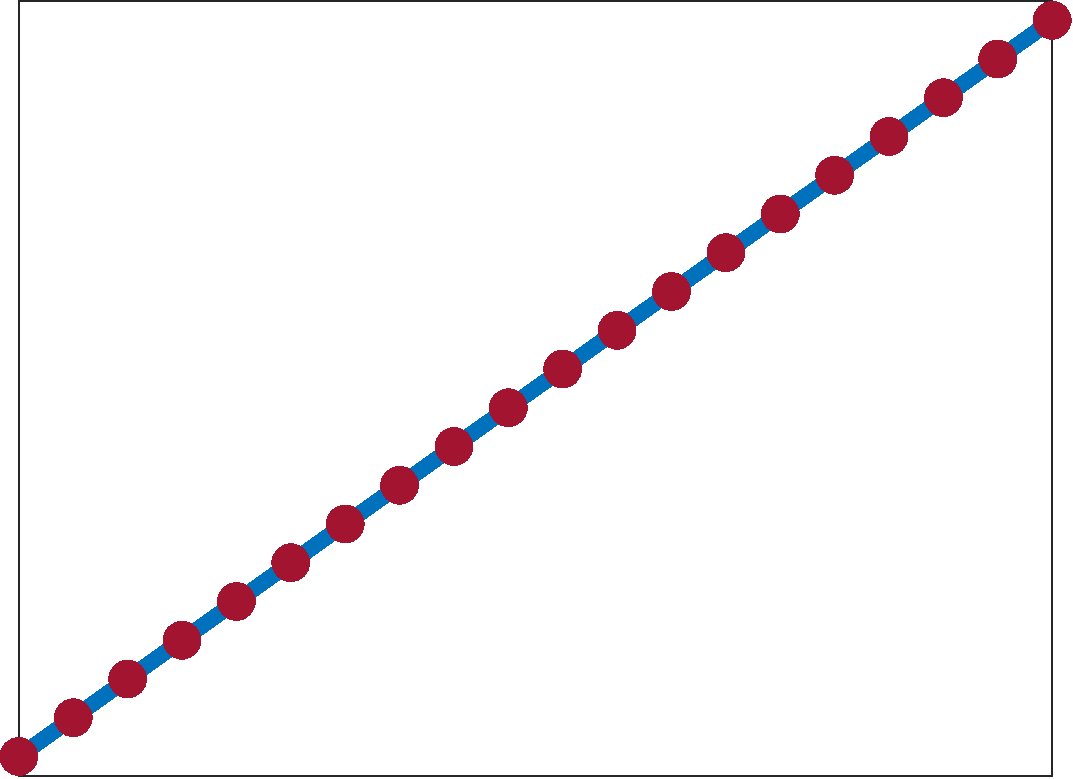
\includegraphics[width=0.16\textwidth]{../src/figures/estimation/gui_linear}}\qquad
\subfloat[Polynomial kernel, $\delta=3$.]{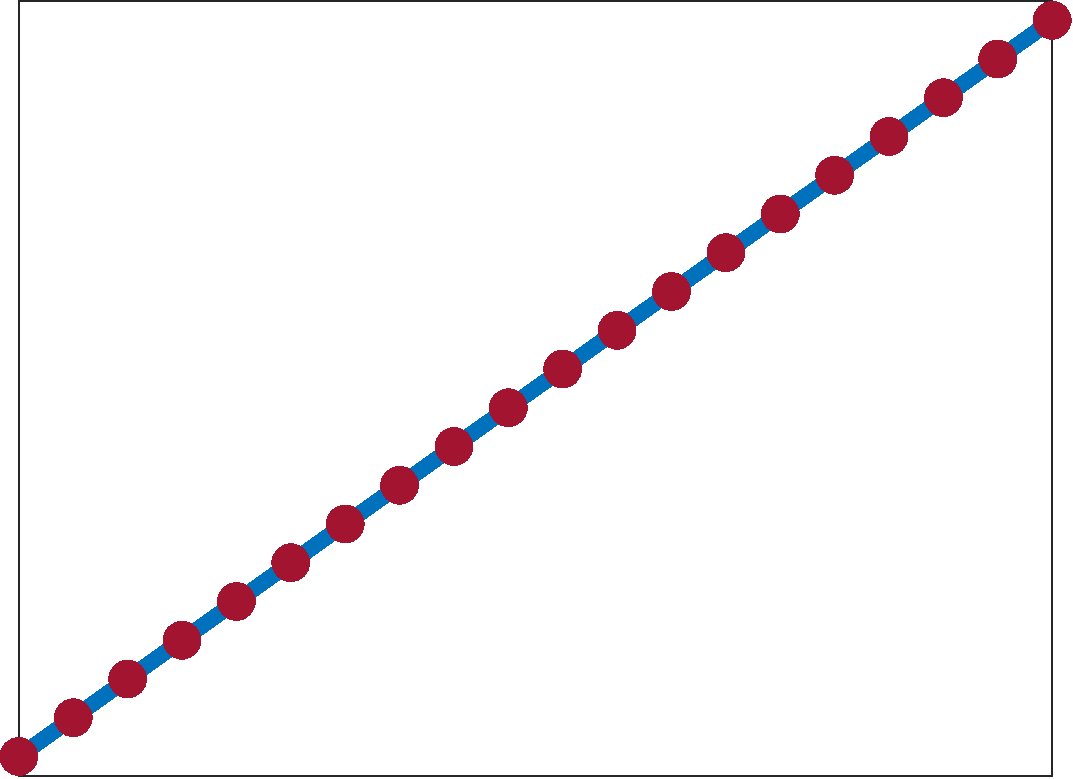
\includegraphics[width=0.16\textwidth]{../src/figures/estimation/gui_polynomial}}\qquad
\subfloat[RBF kernel, $\sigma^2=1$.]{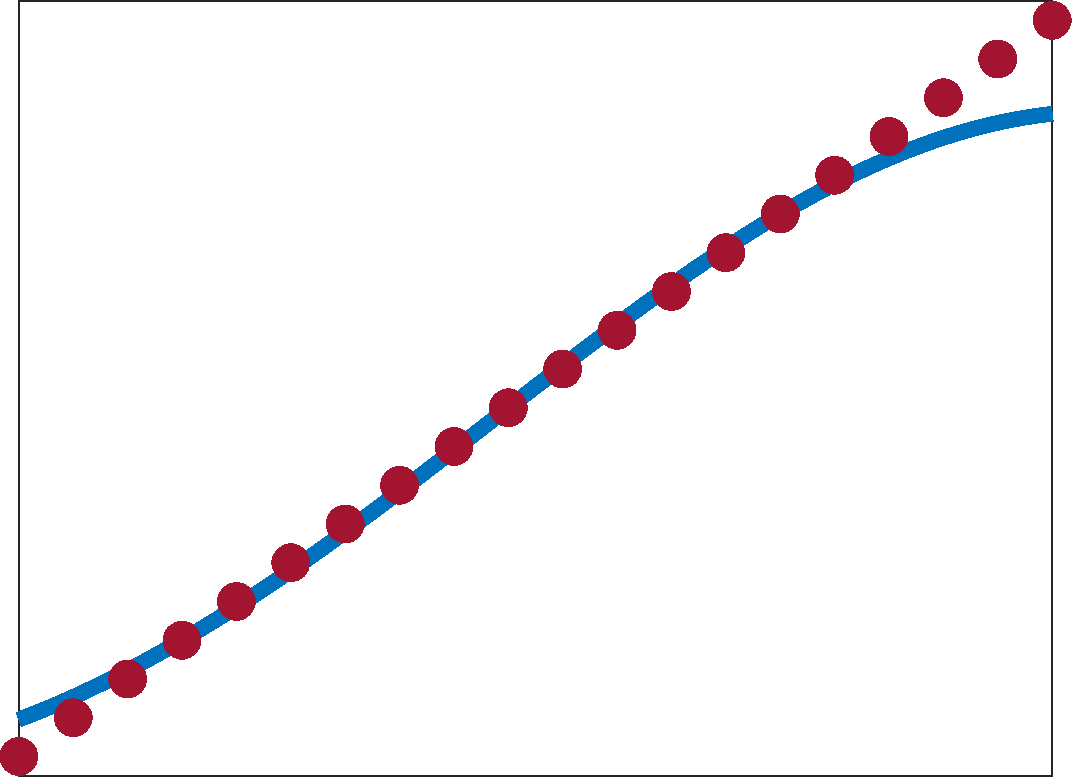
\includegraphics[width=0.16\textwidth]{../src/figures/estimation/gui_rbf}}\qquad
\subfloat[Trigonometric kernel, degree 1.]{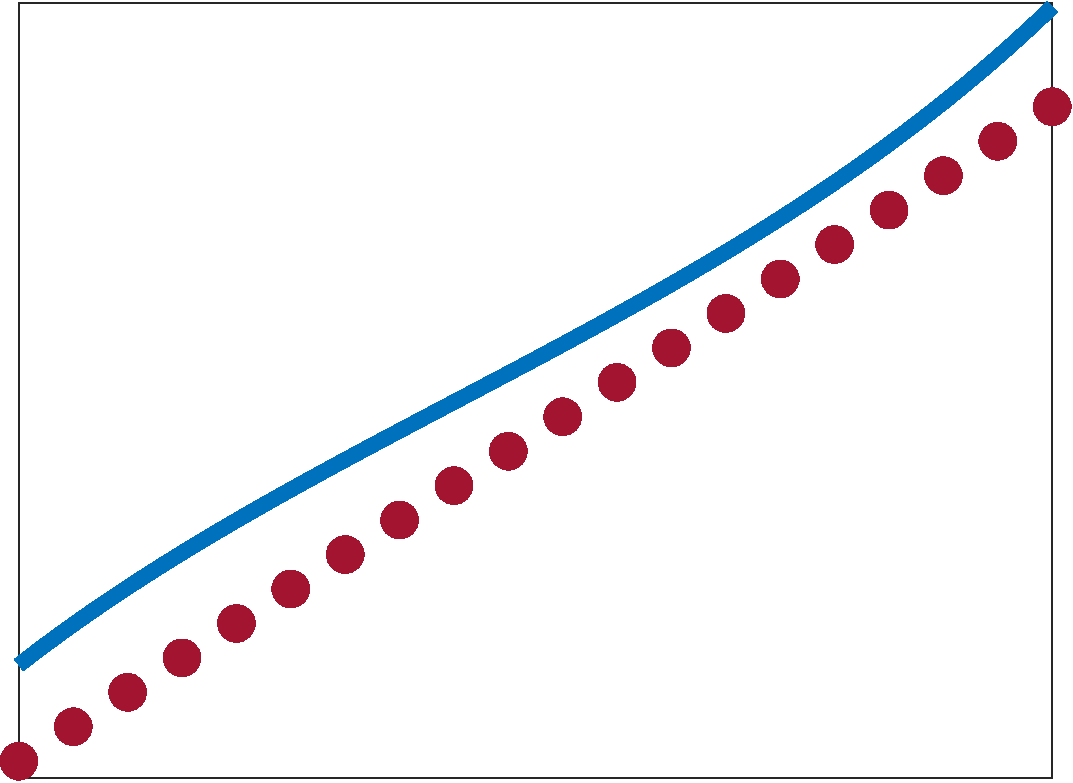
\includegraphics[width=0.16\textwidth]{../src/figures/estimation/gui_trigonometric}}\qquad
\subfloat[Exponential kernel, $\sigma^2=1$.]{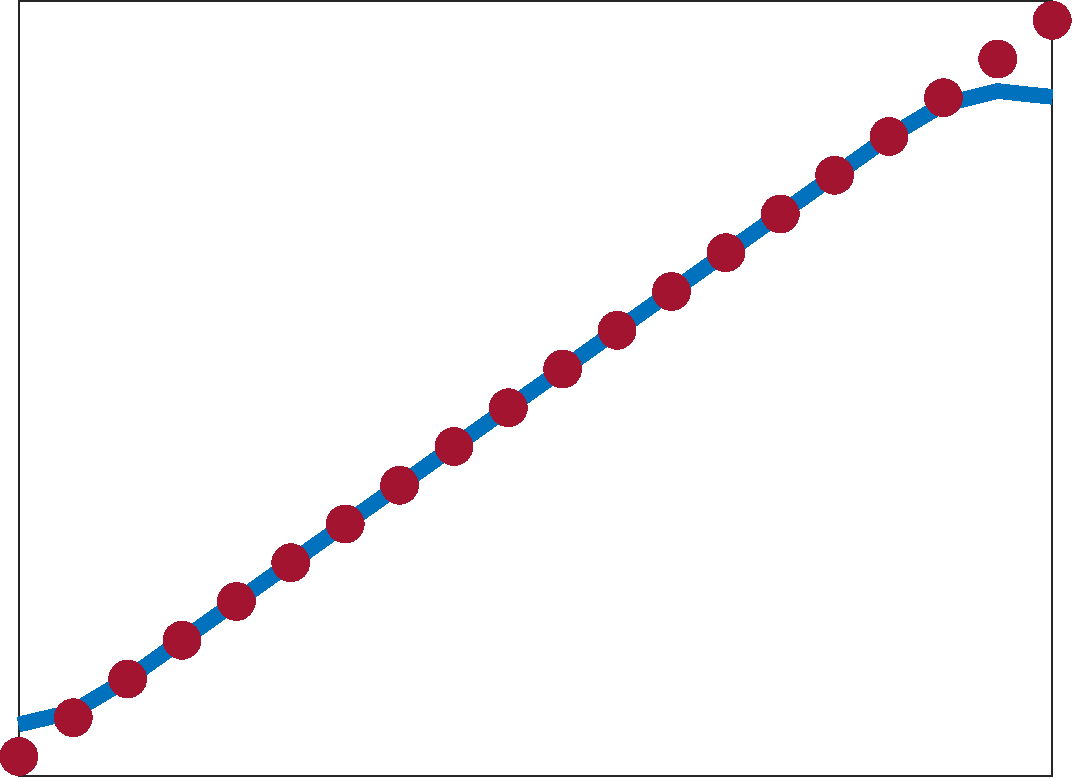
\includegraphics[width=0.16\textwidth]{../src/figures/estimation/gui_exponential}}\qquad
\\
\subfloat[Linear kernel.]{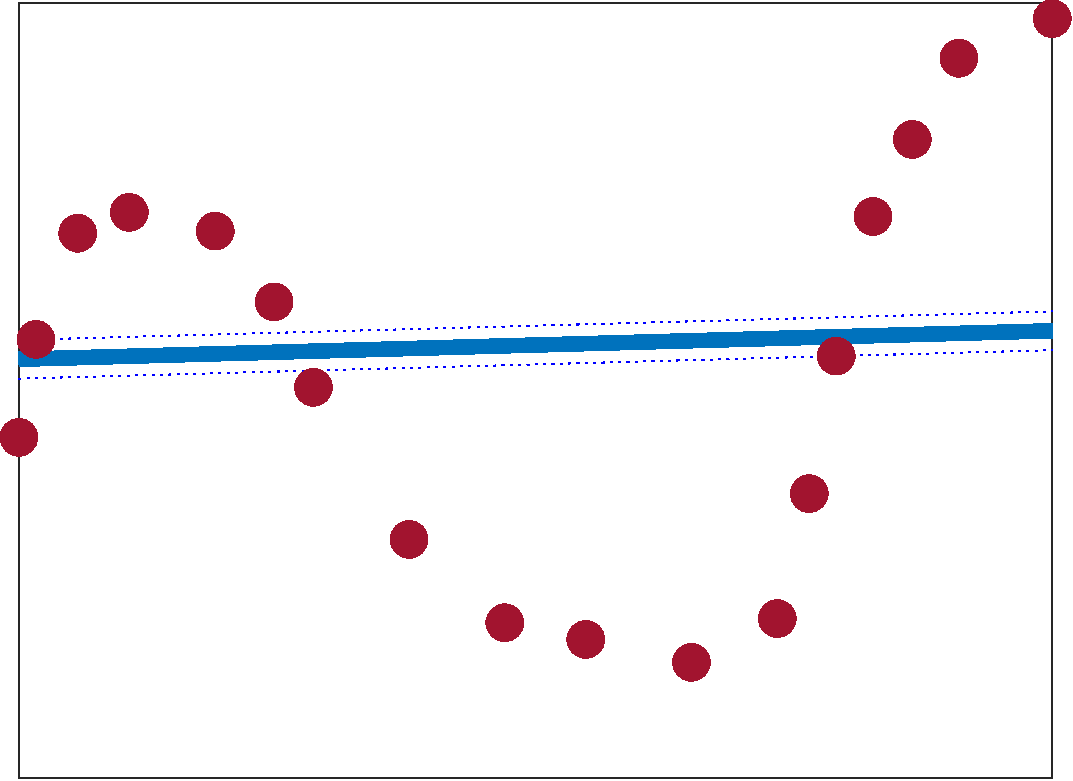
\includegraphics[width=0.16\textwidth]{../src/figures/estimation/gui_nonlinear_linear}}\qquad
\subfloat[Polynomial kernel, $\delta=3$.]{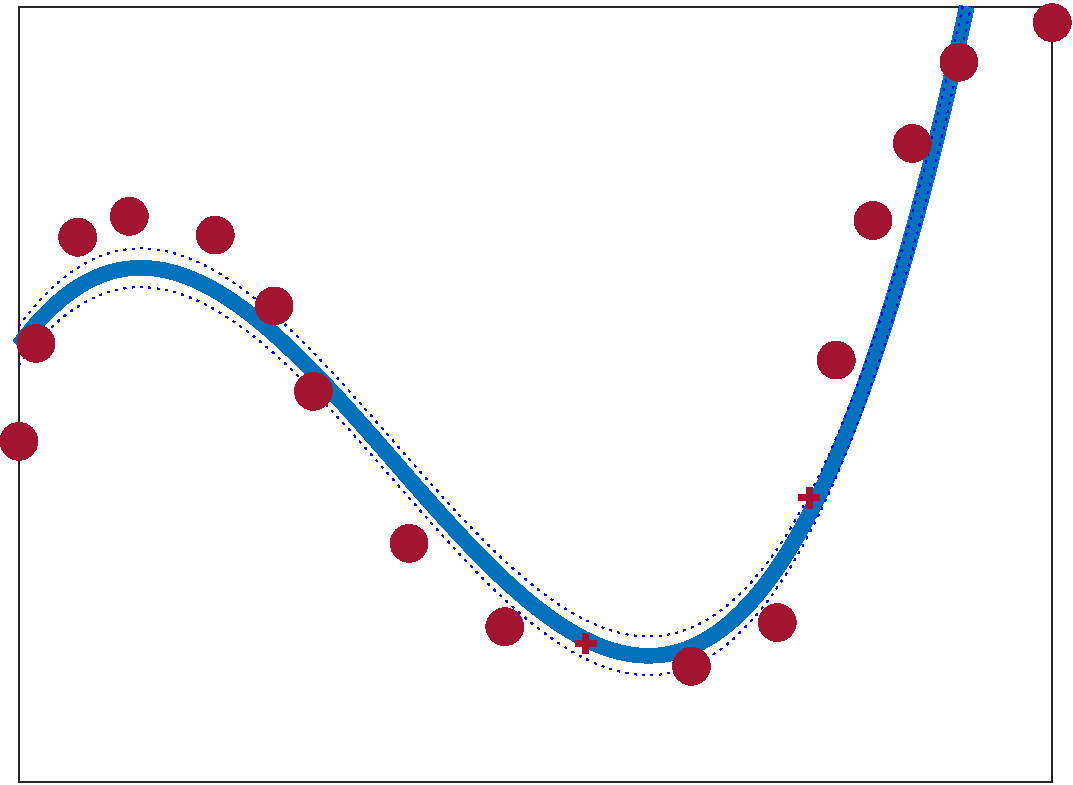
\includegraphics[width=0.16\textwidth]{../src/figures/estimation/gui_nonlinear_polynomial}}\qquad
\subfloat[RBF kernel, $\sigma^2=0.1$.]{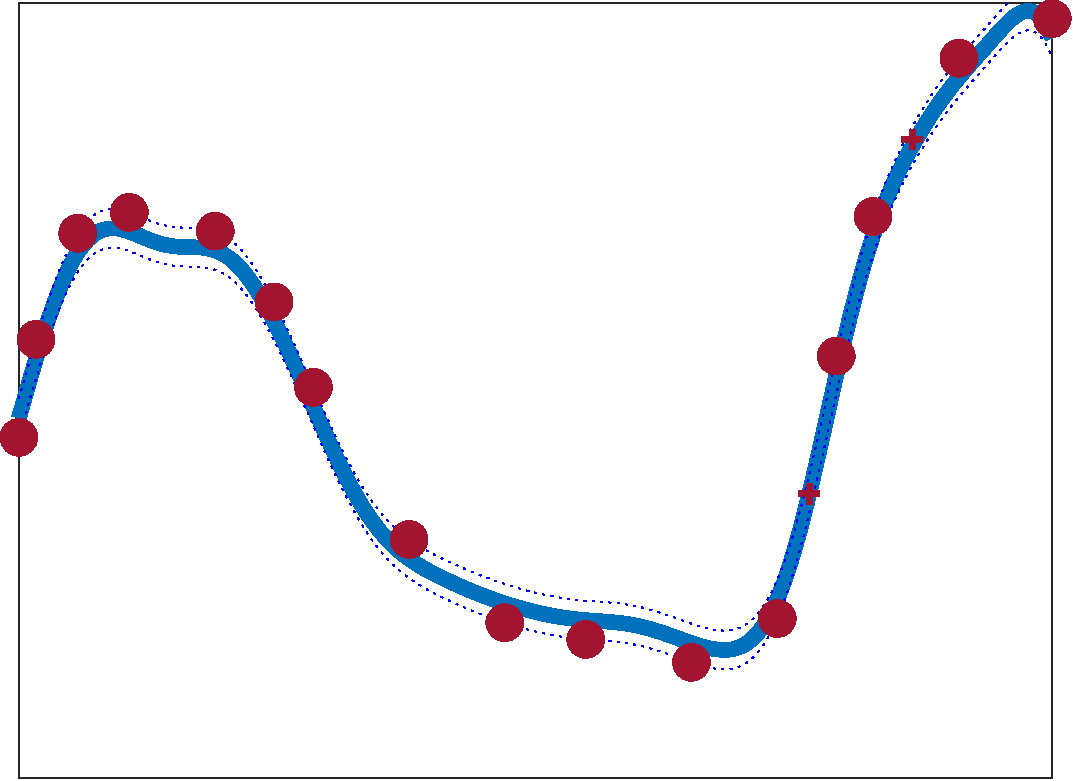
\includegraphics[width=0.16\textwidth]{../src/figures/estimation/gui_nonlinear_rbf}}\qquad
\subfloat[Linear b-spline kernel, degree 5.]{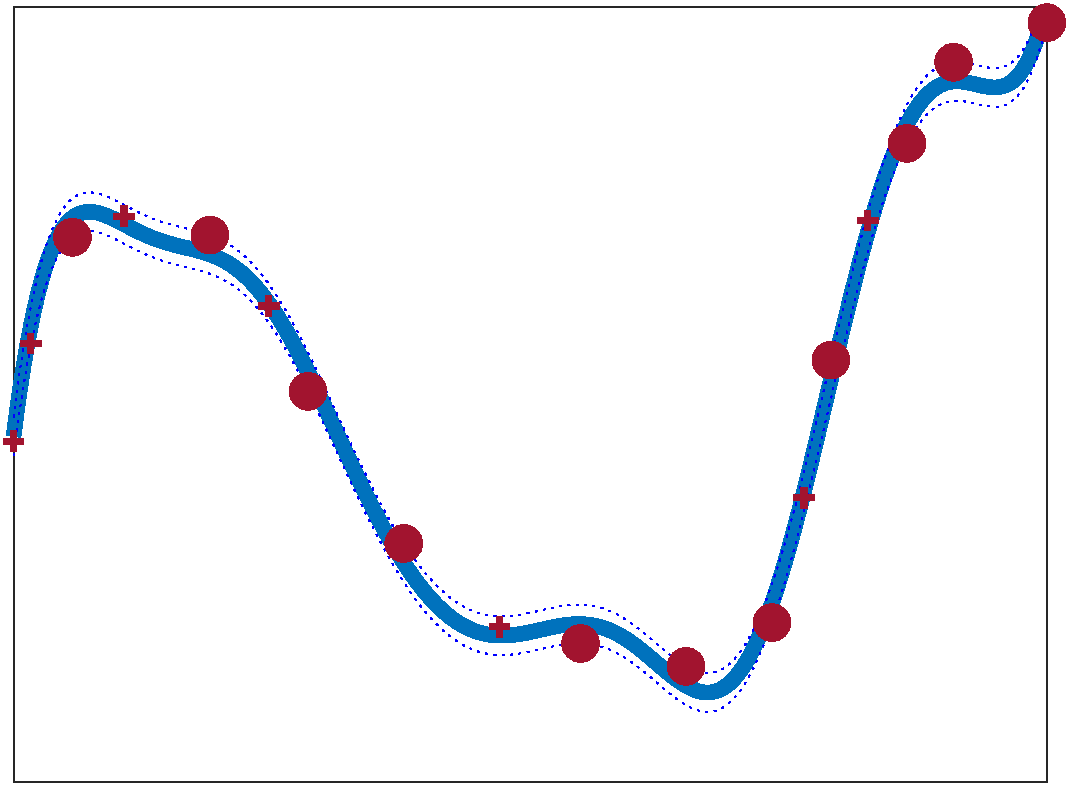
\includegraphics[width=0.16\textwidth]{../src/figures/estimation/gui_nonlinear_bspline}}\qquad
\subfloat[Exponential kernel, $\sigma^2=1.0$.]{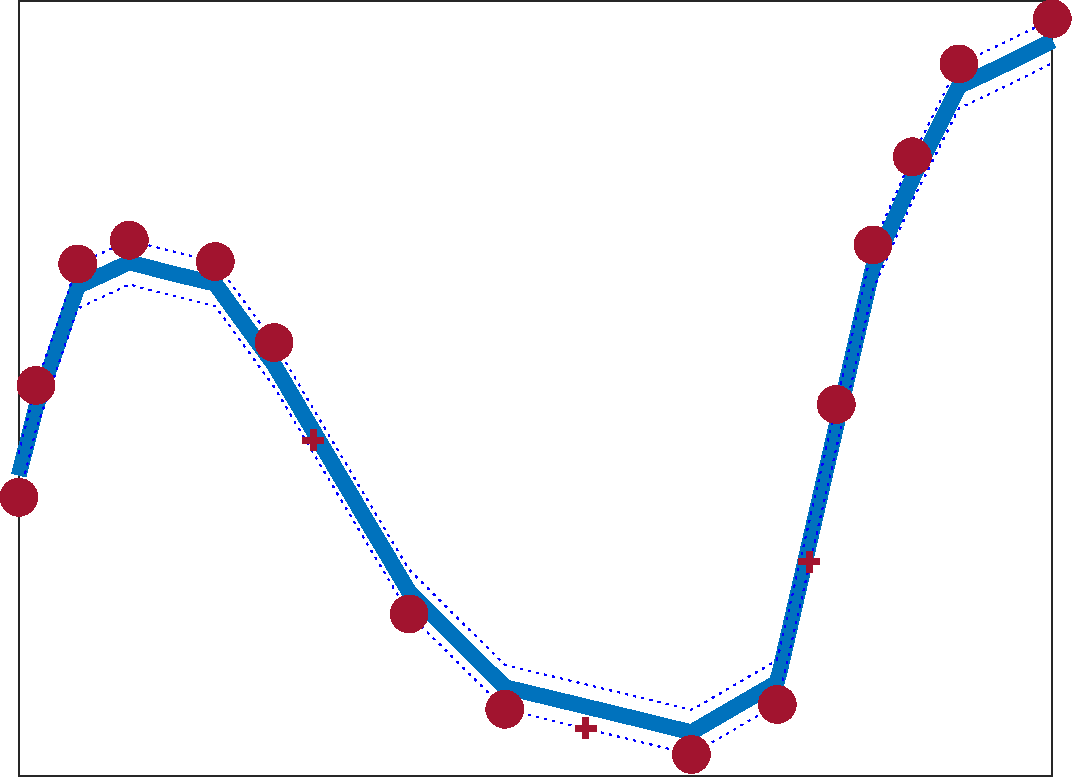
\includegraphics[width=0.16\textwidth]{../src/figures/estimation/gui_nonlinear_exponential}}\qquad
\caption{Visualisation of the results of experiments with various kernels and parameters for two different artificial datasets. In the first row $\epsilon=0$ and \texttt{bound} = 10, in the second one $\epsilon=1$ and \texttt{bound} = 1000. Some of the models are likely to be overfitted though these are just toy examples without any test set.}
\label{functionestimation}
\end{figure}

\fakesubsection{A simple example: the sinc function}{}

Figure \ref{sincestimate} shows the results of LS-SVM regression applied on the \texttt{sinc} function. The mean squared error is lowest for $\sigma^2=1.0,\gamma=10^6$. The smaller $\sigma^2$ value (0.01) leads to overfitting (the noise is being modelled). In this case the underlying function is known and it seems reasonable to take $\sigma\in[0.1,1.0]$ and, say, $\gamma=10^3$. However, an optimal parameter cannot be found as it depends on the training set that is being dealt with and even for a given training set there's no unique parameter combination that works best.

\par Results of automated tuning are shown hereunder :

\begin{table}[h]
\centering
\begin{tabular}{c|ccc}
\textit{Method} & $\gamma$ & $\sigma^2$ & \textit{mean squared error} \\
\hline
Grid search & 5528319.4668 $\pm$ 54371026.5606 & 0.1239 $\pm$  0.1513 & 0.0104 $\pm$ 0.0001\\
Nelder-Mead & 2329.7378 $\pm$ 2318.2696 & 0.1049 $\pm$ 0.0892 &  0.0104 $\pm$ 0.0001\\
\end{tabular}
\caption{Results of automated tuning strategies (averaged over 40 runs).}
\label{automatedtuning}
\end{table}

The results are comparable to those obtained previously in the context of classification, with a few outliers for $\gamma$. Again, grid search appeared to be slower (185 seconds versus 110 for the simplex method). Some of the models seem to overfit the data a bit.

\begin{figure}[h]
\centering
\subfloat[$\gamma=10,\sigma=0.01,\rho=0.0117$]{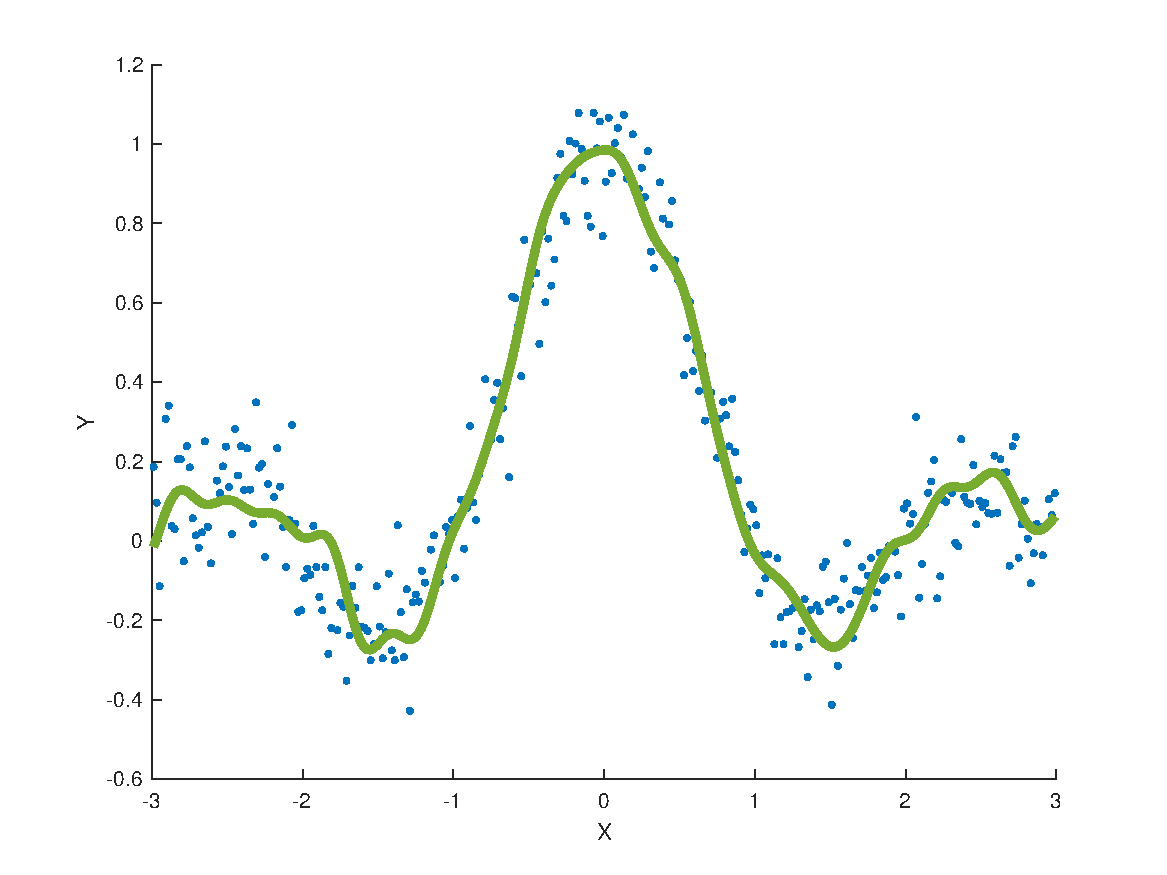
\includegraphics[width=0.3\textwidth]{../src/figures/estimation/regression_1}}\qquad
\subfloat[$\gamma=10,\sigma=1,\rho=0.0296$]{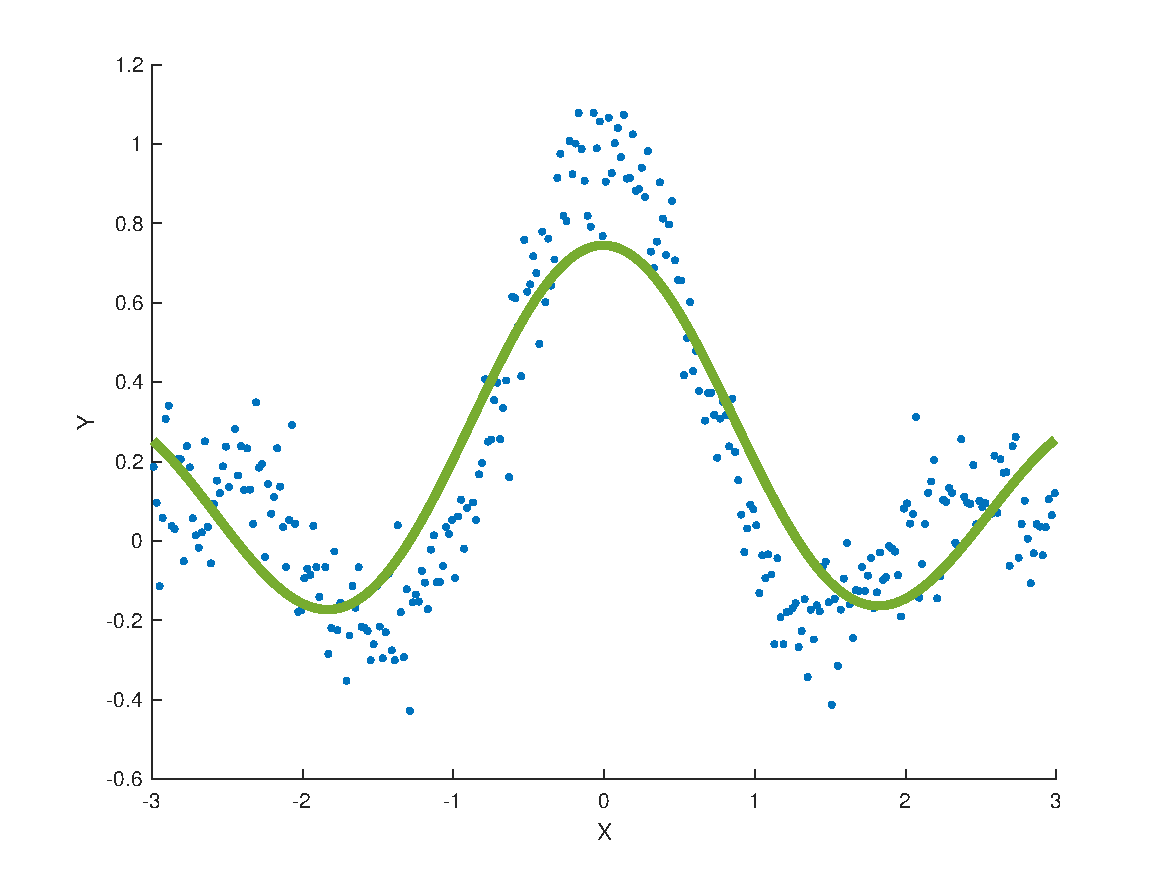
\includegraphics[width=0.3\textwidth]{../src/figures/estimation/regression_2}}\qquad
\subfloat[$\gamma=10,\sigma=100,\rho=0.1273$]{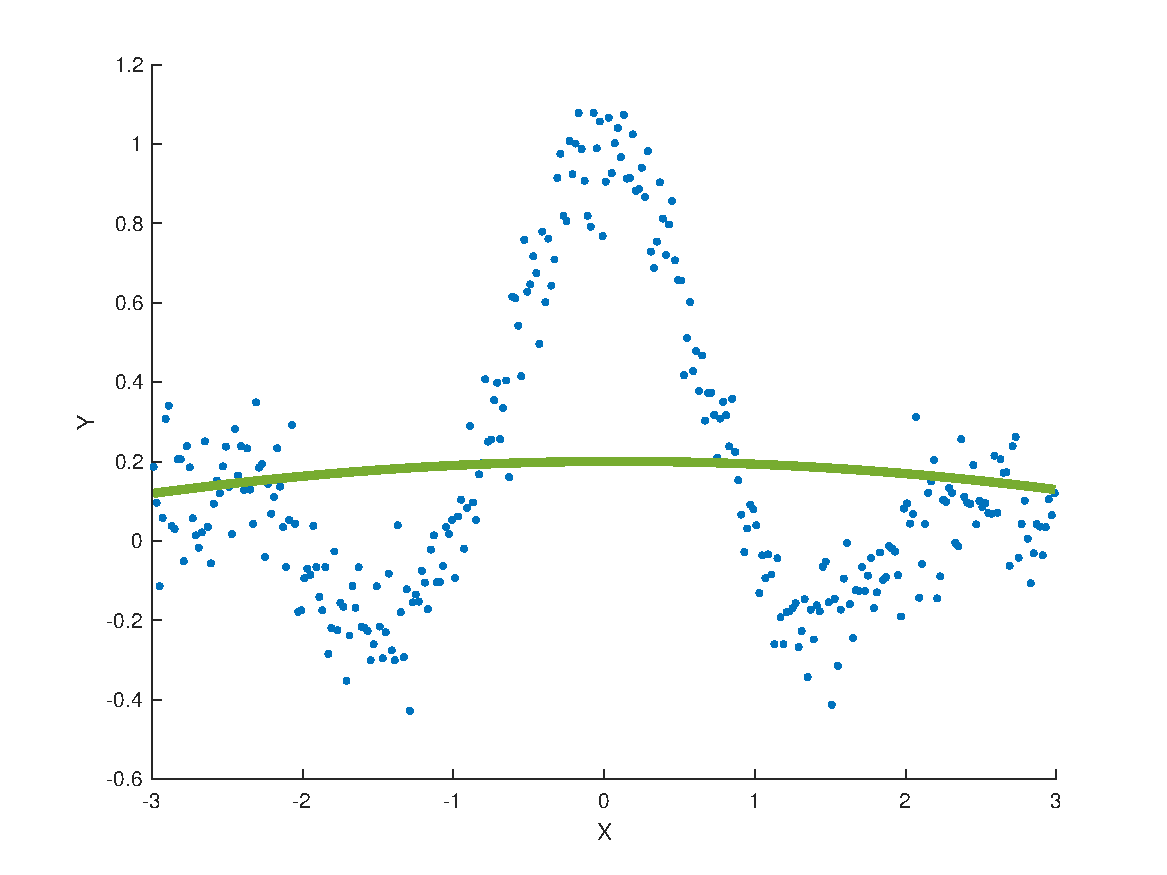
\includegraphics[width=0.3\textwidth]{../src/figures/estimation/regression_3}}\qquad
\\
\subfloat[$\gamma=10^3,\sigma=0.01,\rho=0.0120$]{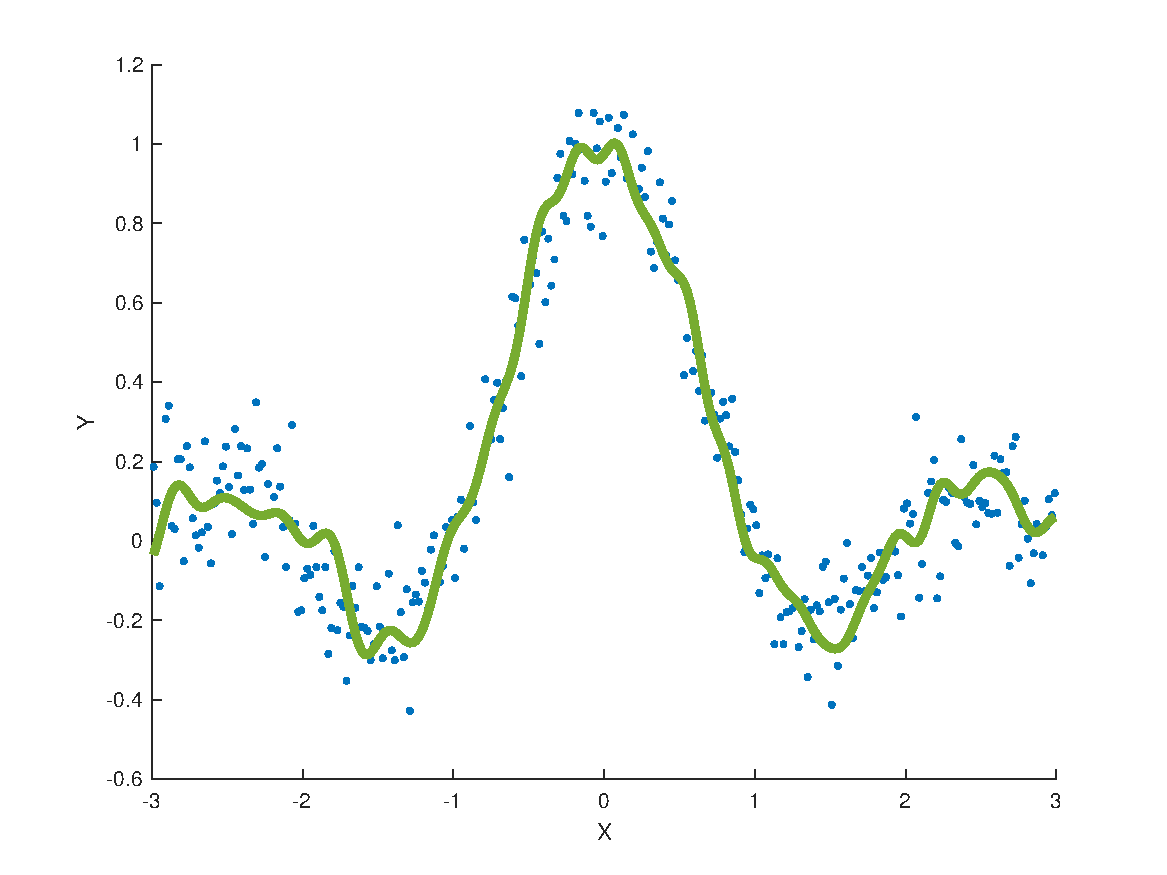
\includegraphics[width=0.3\textwidth]{../src/figures/estimation/regression_4}}\qquad
\subfloat[$\gamma=10^3,\sigma=1,\rho=0.0114$]{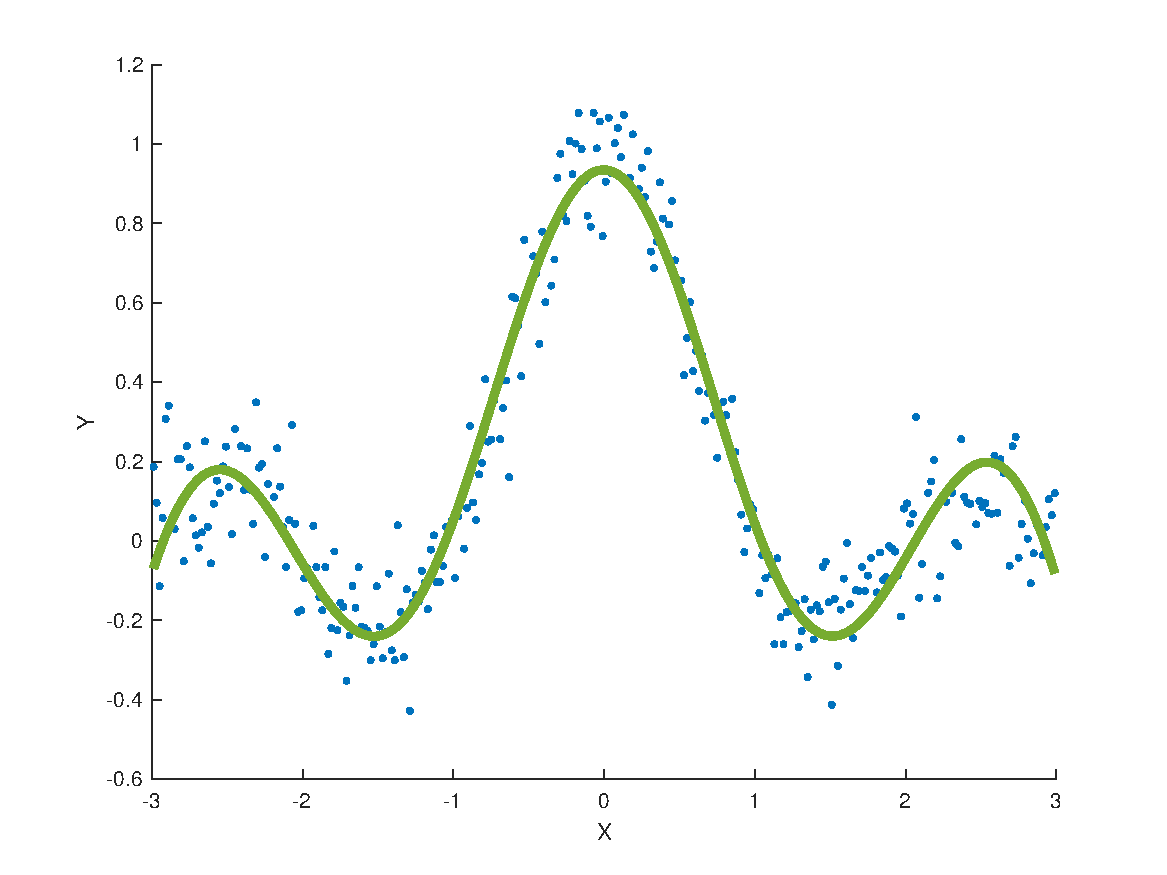
\includegraphics[width=0.3\textwidth]{../src/figures/estimation/regression_5}}\qquad
\subfloat[$\gamma=10^3,\sigma=100,\rho=0.1107$]{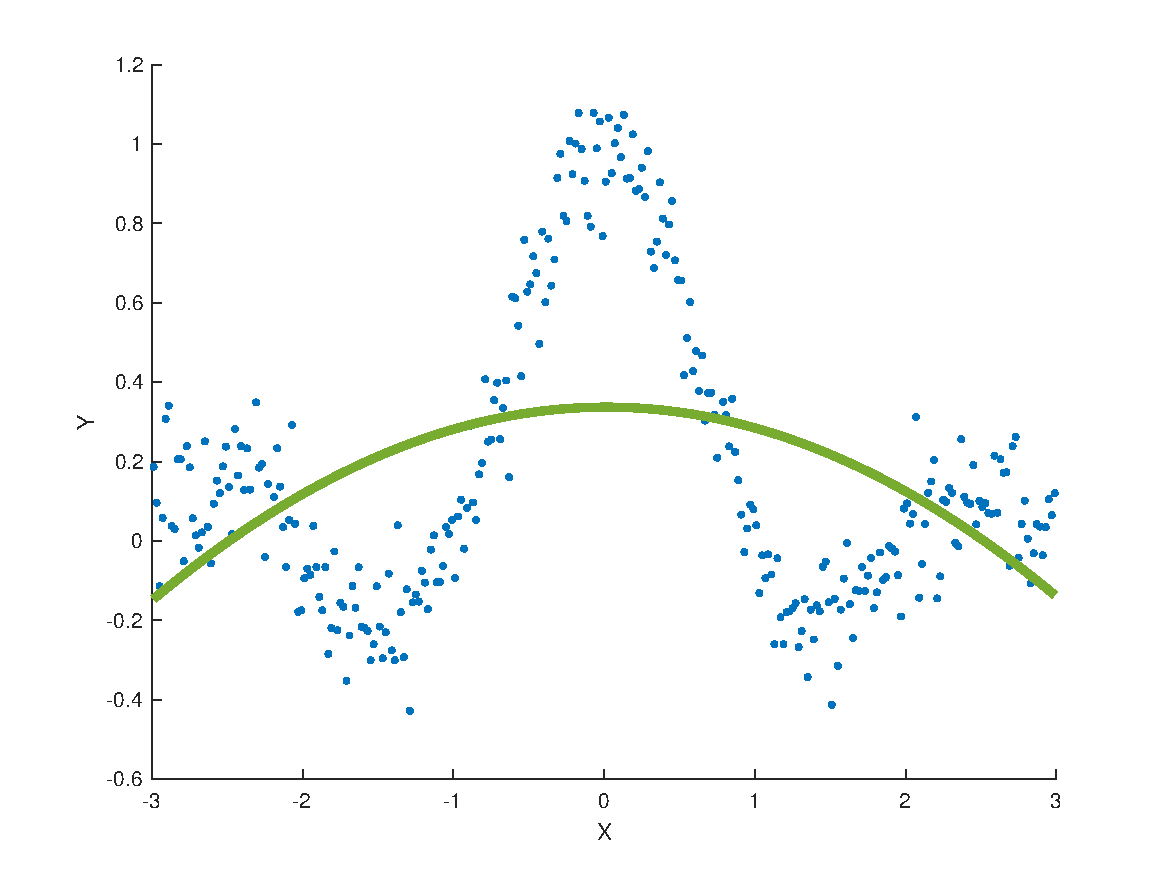
\includegraphics[width=0.3\textwidth]{../src/figures/estimation/regression_6}}\qquad
\\
\subfloat[$\gamma=10^6,\sigma=0.01,\rho=0.0125$]{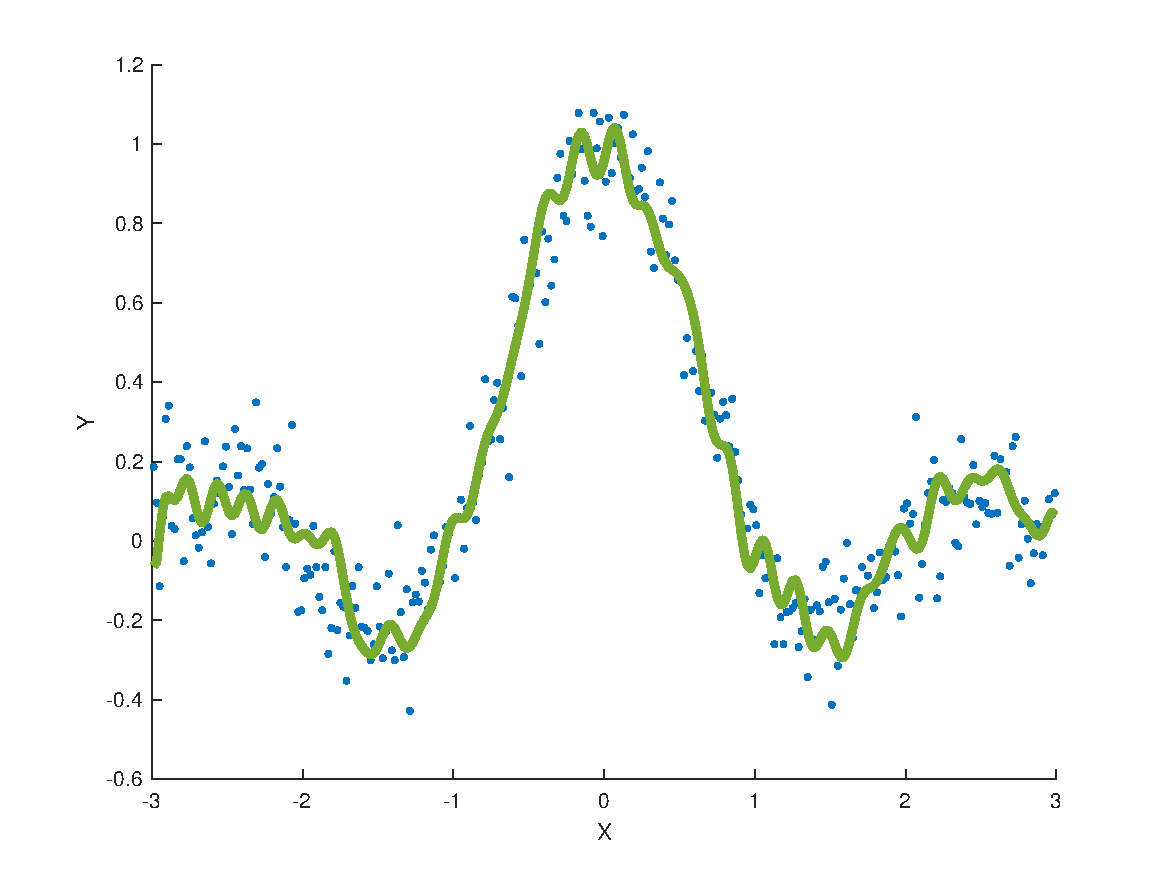
\includegraphics[width=0.3\textwidth]{../src/figures/estimation/regression_7}}\qquad
\subfloat[$\gamma=10^6,\sigma=1,\rho=0.0099$]{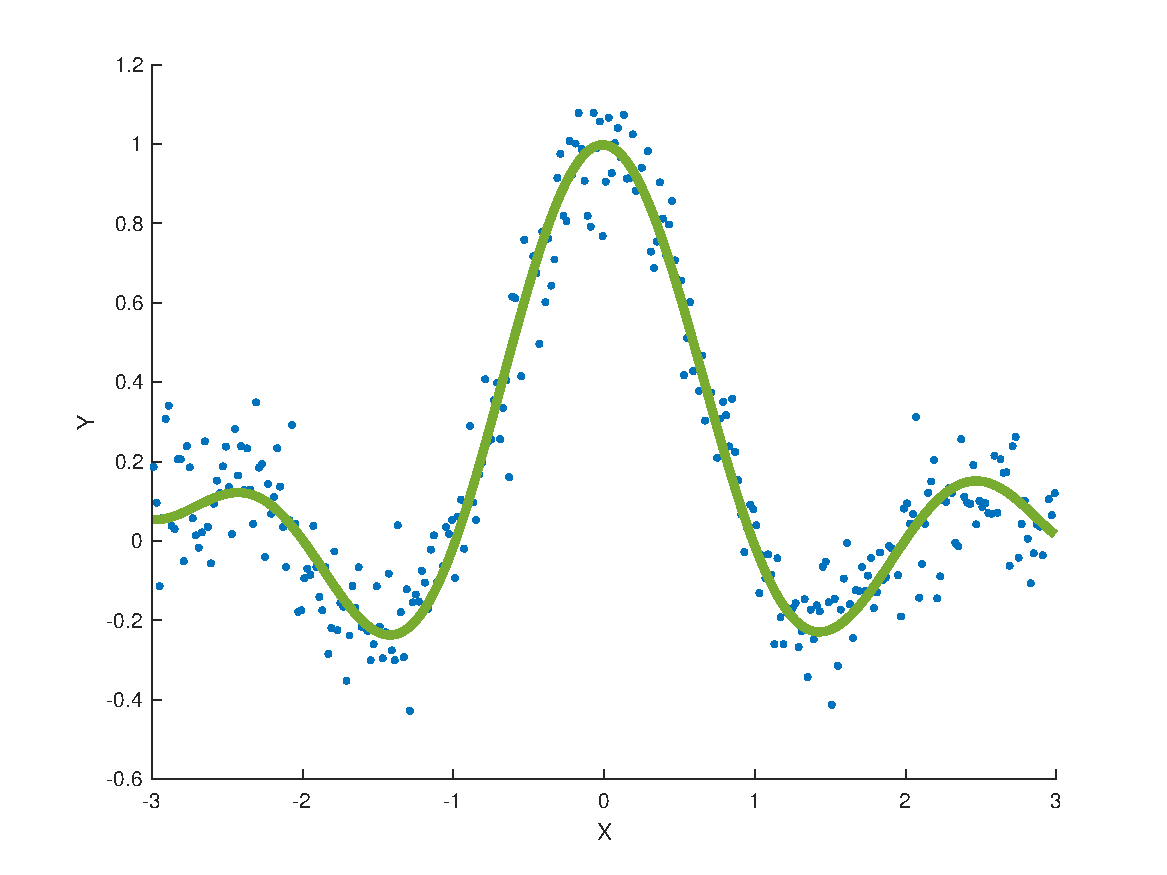
\includegraphics[width=0.3\textwidth]{../src/figures/estimation/regression_8}}\qquad
\subfloat[$\gamma=10^6,\sigma=100,\rho=0.1048$]{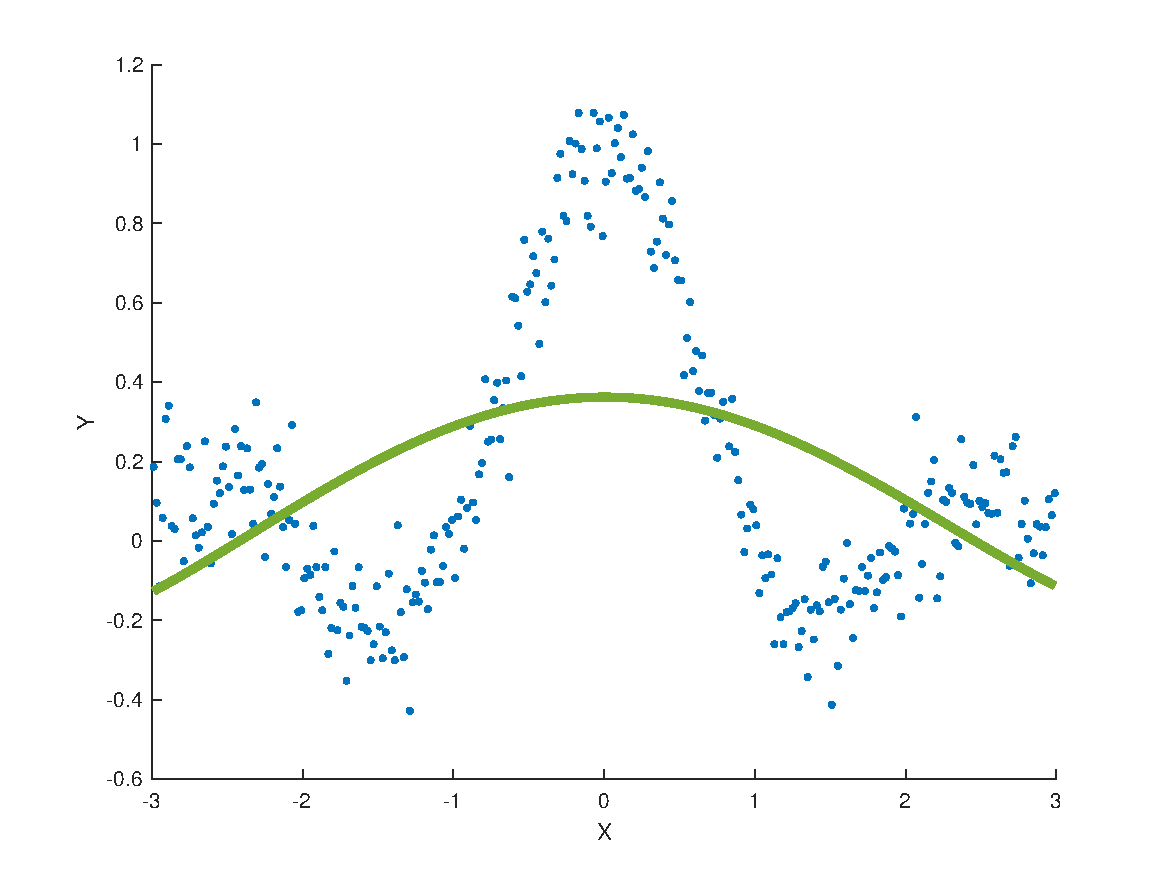
\includegraphics[width=0.3\textwidth]{../src/figures/estimation/regression_9}}\qquad
\caption{Function estimation experiments with the \texttt{sinc} function. Noisy samples are fed to an LS-SVM. The green line is the estimated model, the blue dots represent the test data. $\rho$ is the mean squared error. Small $\sigma$ values make the model fit the noise.}
\label{sincestimate}
\end{figure}

When making use of a validation set that very set cannot be used for training. Making use of a Bayesian framework is an alternative and allows one to infer appropriate parameter combinations while making full use of the dataset. Depending on the kernel that is being used either 2 or 3 levels of inference are applied. At each of these level Bayes' theorem is used to infer parameter values. The equations are : 

\begin{equation}
p(\textbf{w},\textbf{b}|\mathcal{D},\mu,\zeta_{1\_N},\mathcal{H}_{\sigma}) = \frac{p(\mathcal{D}|w,b,\mu,\zeta_{1\_N},\mathcal{H}_{\sigma})}{\textcolor{cyan}{p(\mathcal{D}|\mu,\zeta_{1\_N},\mathcal{H}_{\sigma})}}\cdot p(w,b|\mu,\zeta_{1\_N},\mathcal{H}_{\sigma})
\end{equation}
\begin{equation}
p(\boldsymbol{\mu},\boldsymbol{\zeta_{1\_N}}|\mathcal{D},\mathcal{H}_{\sigma})=\frac{\textcolor{cyan}{p(\mathcal{D}|\mu,\zeta_{1\_N},\mathcal{H}_{\sigma})}}{\textcolor{teal}{p(\mathcal{D}|\mathcal{H}_{\sigma})}}\cdot p(\mu,\zeta_{1\_N}|\mathcal{H}_{\sigma})
\end{equation}
\begin{equation}
p(\boldsymbol{\mathcal{H}_{\sigma}}|\mathcal{D})=\frac{\textcolor{teal}{p(\mathcal{D}|\mathcal{H}_{\sigma})}}{p(D)}\cdot p(\mathcal{H}_{\sigma})
\end{equation}

As indicated by the colourings the evidence at any level equals the likelihood in the next level. At the first level one can take the logarithm of the product to see the relation with the primal form in the LS-SVM problem specification ; while the prior corresponds to the regularisation term the likelihood corresponds to the least squares cost term.

\begin{figure}[h]
    \centering
    \begin{minipage}{0.45\textwidth}
        \centering
        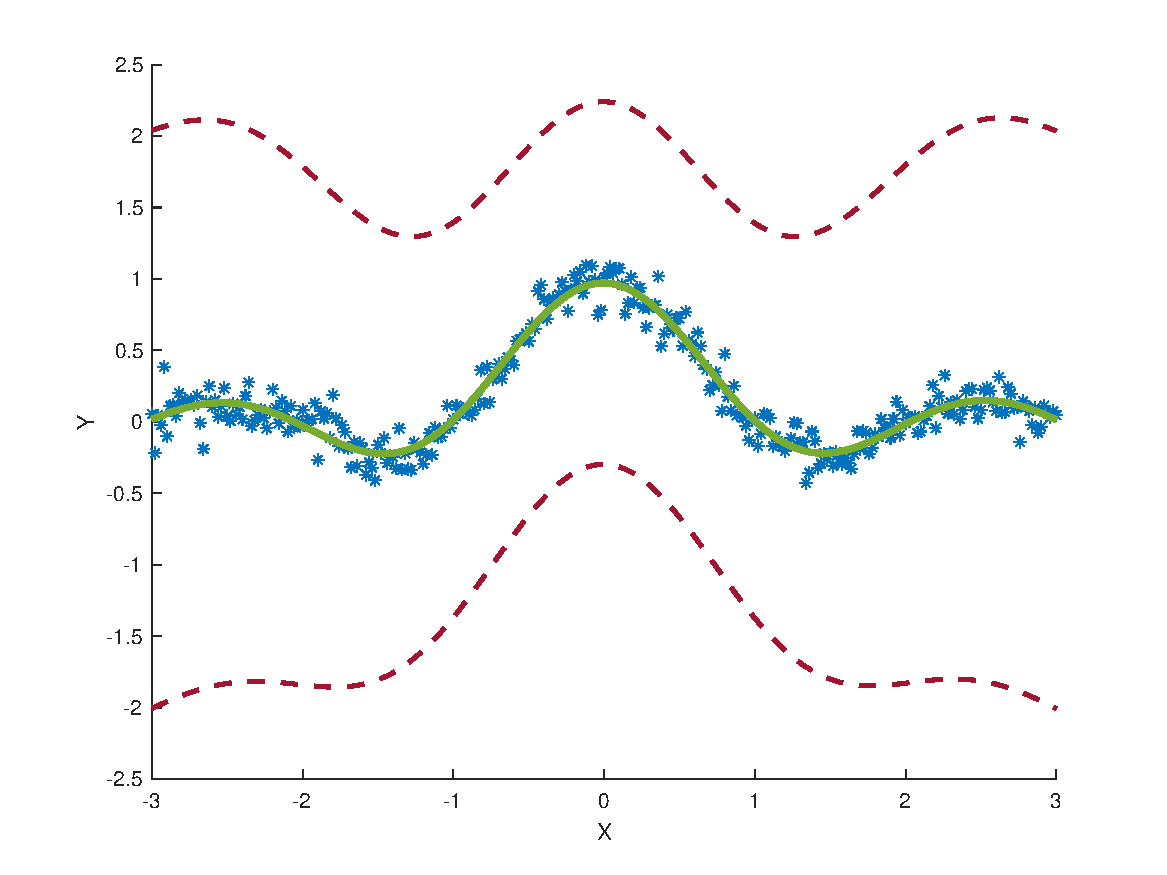
\includegraphics[width=0.9\textwidth]{../src/figures/estimation/bayesian_inference}
        \caption{Results of Bayesian inference applied on training data based on the \texttt{sinc} function with some added white noise (blue). The function estimate is coloured in green, 95\% error bars are indicated in red.}
\label{bayesianinference}
    \end{minipage}\hfill
    \begin{minipage}{0.45\textwidth}
        \centering
        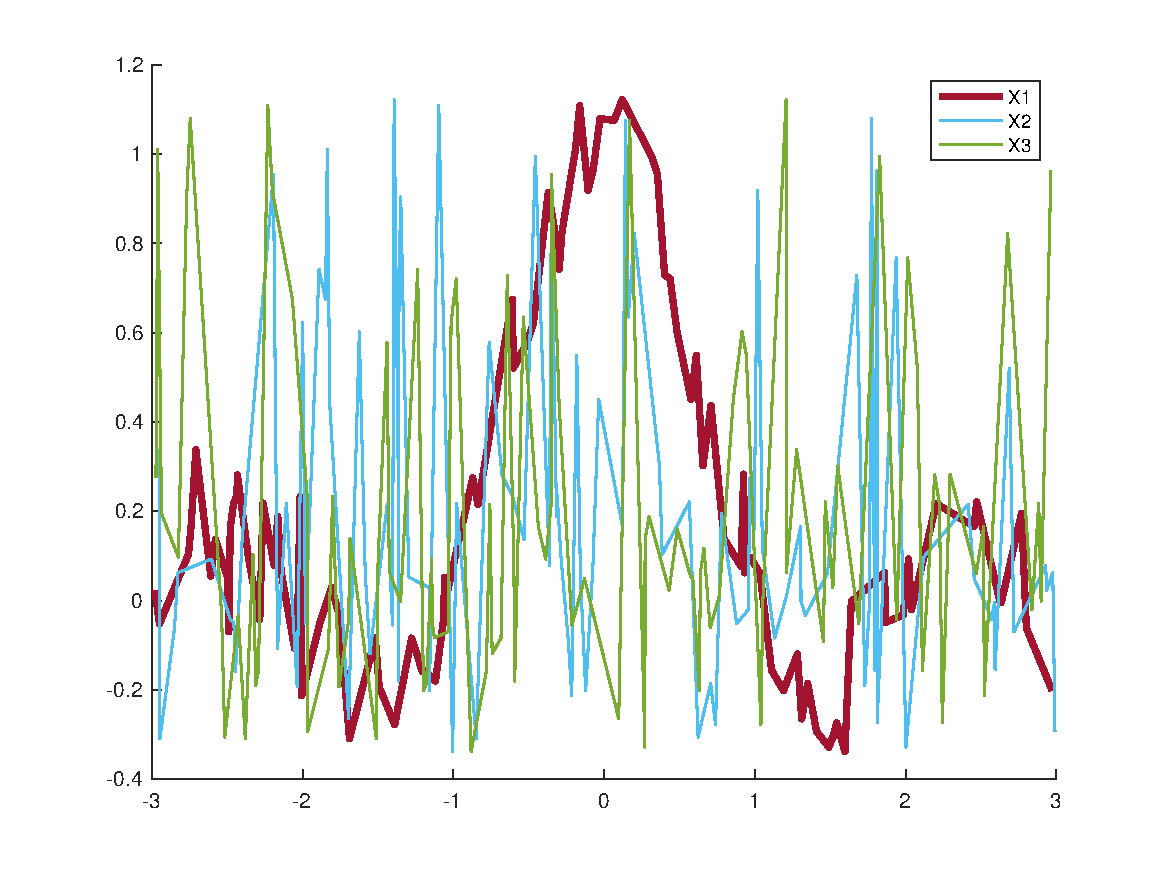
\includegraphics[width=0.9\textwidth]{../src/figures/estimation/ard}
        \caption{Plot of 3-dimensional input data of which only the first dimension models the \texttt{sinc} function, the other 2 being white noise.}
\label{ardsinc}
    \end{minipage}
\end{figure}

One nice facet of this approach is that one ends up with error bars indicating uncertainty of the prediction. These error bars can be seen in figure \ref{bayesianinference} where the method is applied on the \texttt{sinc} function.

\fakesubsection{Automatic relevance determination (ARD)}{}

By modifying the kernel function for the LS-SVM dual formulation it becomes possible to disregard irrelevant or noisy input dimensions when these don't contribute to the final classification (a form of dimensionality reduction). In the case of an RBF kernel by using a diagonal matrix $S$ as a weighted norm a bandwidth is associated with each of the input dimensions. Level 3 of the Bayesian framework discussed before is then used to infer the elements of $S$ and any input dimensions associated with small bandwidths are iteratively disregarded until no additional improvement is obtained. For the toy dataset the algorithm found $x_1$ to be the sole relevant one which is also illustrated in figure \ref{ardsinc}. An other, crude way of doing relevance determination is to consider all possible non-empty subsets of the input features and applying cross-validation on the resulting data to figure out which subset generalises best. For the given data the conclusion remained the same as any subset excluding the first (non-noisy) dimension performed badly ($mse>0.1$) and the subset excluding all but the first dimensions performed best ($mse\approx 0.012$). This method wouldn't be satisfactory in practice as the power set grows sharply as the number of input dimensions increases. Treating the problem as a global optimisation is more appropriate for example. Or even simply removing random features one by one as long as the results keep on improving.

\fakesubsection{Robust regression}{}

Two downsides of LS-SVMs are the loss of sparsity and the lack of robustness. Outliers can increase the variance of the decision boundary quite a bit due to the use of the least squares loss, which penalises outliers more than the \textit{mean absolute error} does due to its gradient (such that there is more perturbation). If the noise on the data set is Gaussian then the least squares loss is appropriate, but in general the distribution of the noise is not known and in the case of the toy dataset dealt with here the noise isn't normally distributed. The idea, then, is to find an LS-SVM model as per usual and apply methods from robust statistics on the resulting parameters. Specifically, a weight is assigned to each data point based on its error. Some possible weight functions are shown below. 

\par After assigning the weights a weighted LS-SVM is trained and the whole process may be repeated as desired. Results with 4 weight functions are compared with a non-robust LS-SDM approach in figure \ref{robustsinc}.
\vspace{0.4cm}
\begin{table}[h]
\centering
\begin{tabular}{c|cccc}
& \textit{Huber} & \textit{Hampel} & \textit{Logistic} & \textit{Myriad}\\
\hline
\textit{Weight function} $W(r)$ & $\begin{cases}1\quad\text{if}\ |r|<\beta\\\frac{\beta}{|r|}\quad\text{if}\ |r|\geq\beta\end{cases}$ & $\begin{cases}1\quad\text{if}\ |r|<\beta_1\\\frac{b_2-|r|}{b_2-b_1}\quad\text{if}\ \beta_1\leq|r|\leq\beta_2\\0\quad\text{if}\ |r|>\beta_2\end{cases}$ & $\frac{tanh(r)}{r}$ & $\frac{\delta^2}{\delta^2+r^2}$\\
\end{tabular}
\caption{Possible weight functions for use in robust regression with LS-SVMs.}
\label{roburegwf}
\end{table}

\begin{figure}[h]
\centering
\subfloat[Non-robust regression.]{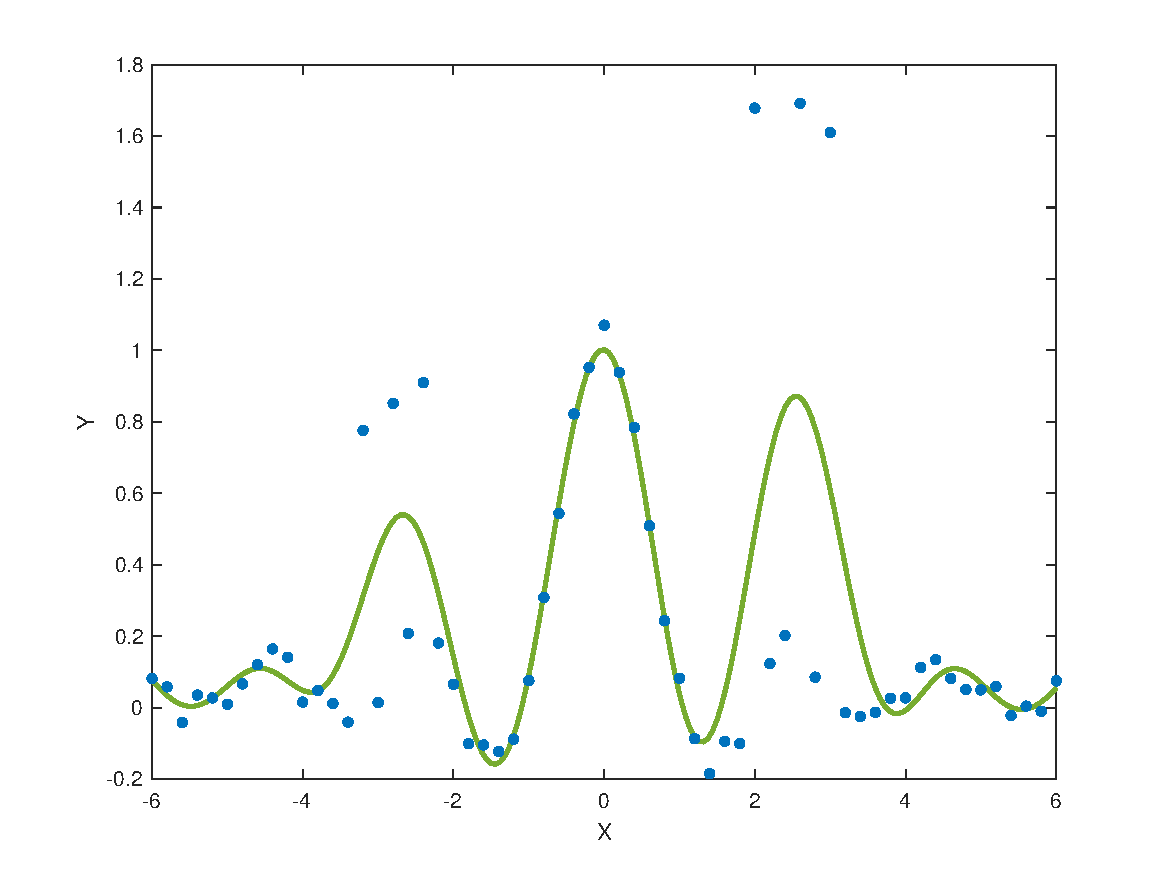
\includegraphics[width=0.3\textwidth]{../src/figures/estimation/robustregression_non}}\qquad
\subfloat[Error values for the non-robust regression ($\frac{\alpha_k}{\gamma}$). After robust regression the errors decrease for the non-outliers which means that aside from those 6 outliers at the top the remaining values are centered around the x-axis.]{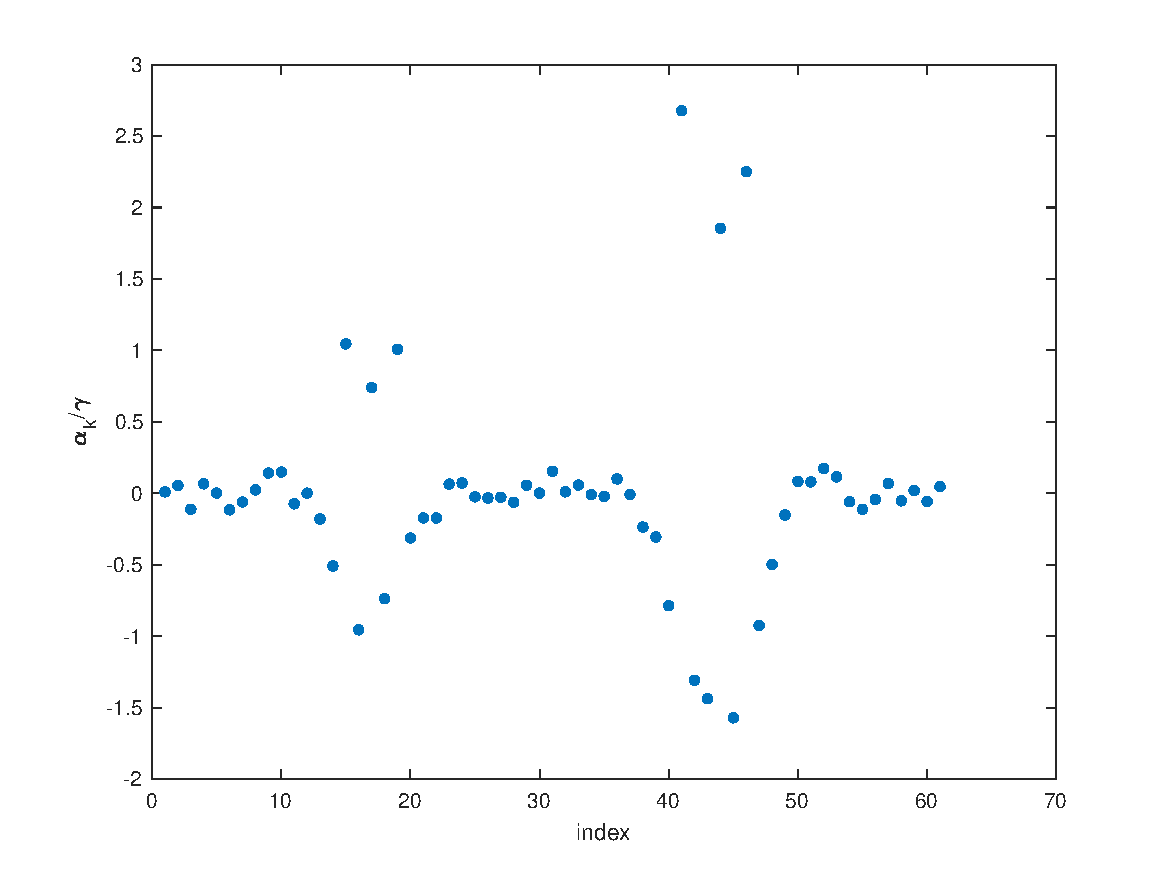
\includegraphics[width=0.3\textwidth]{../src/figures/estimation/robustregression_non_alpha}}
\\
\subfloat[\textit{Huber} weight function.]{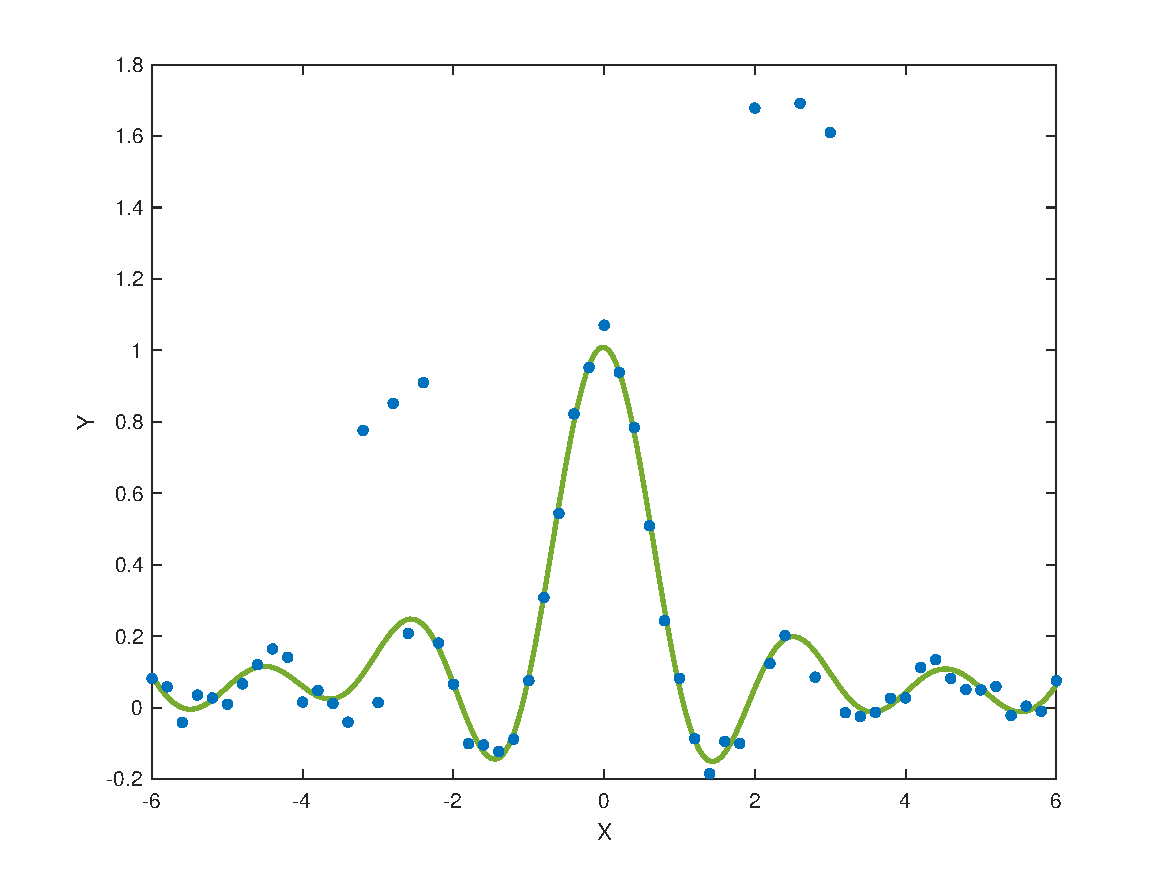
\includegraphics[width=0.3\textwidth]{../src/figures/estimation/robustregression_whuber}}\qquad
\subfloat[\textit{Hampel} weight function.]{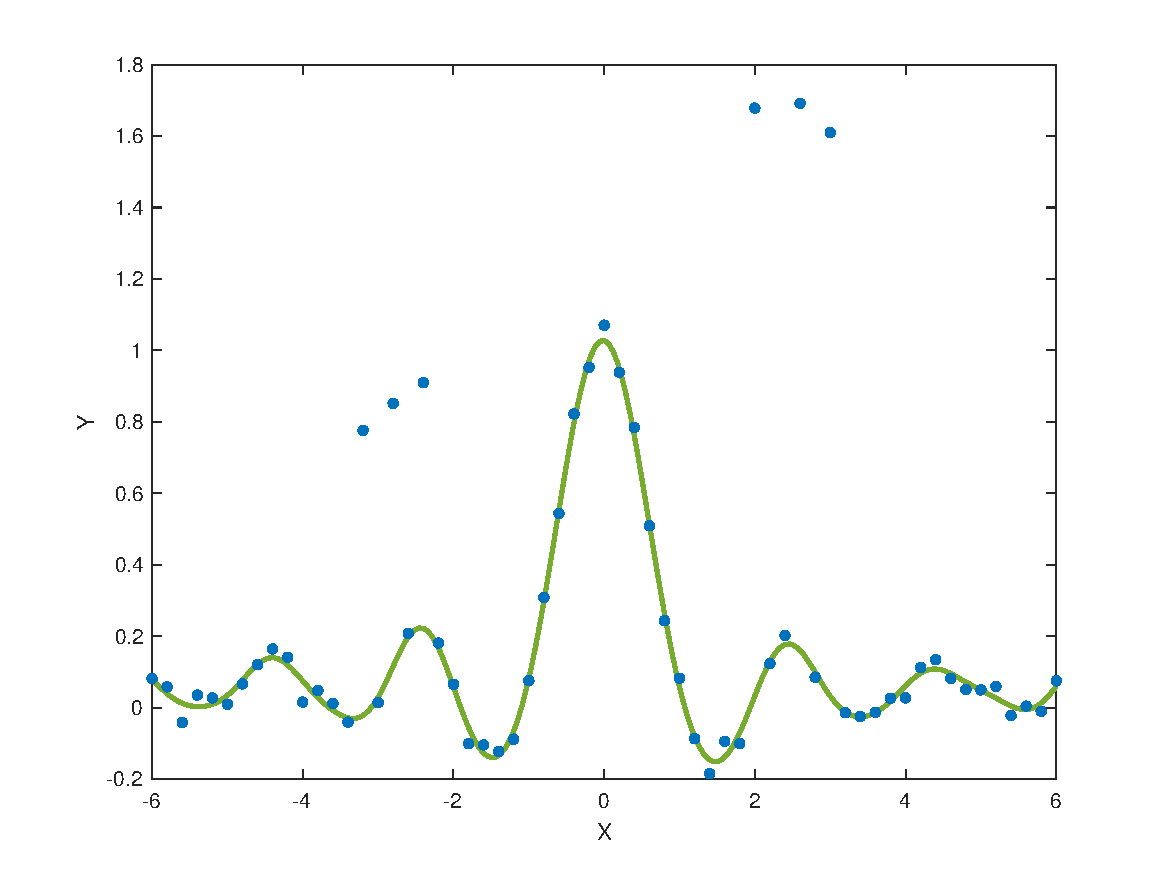
\includegraphics[width=0.3\textwidth]{../src/figures/estimation/robustregression_whampel}}
\\
\subfloat[\textit{Logistic} weight function.]{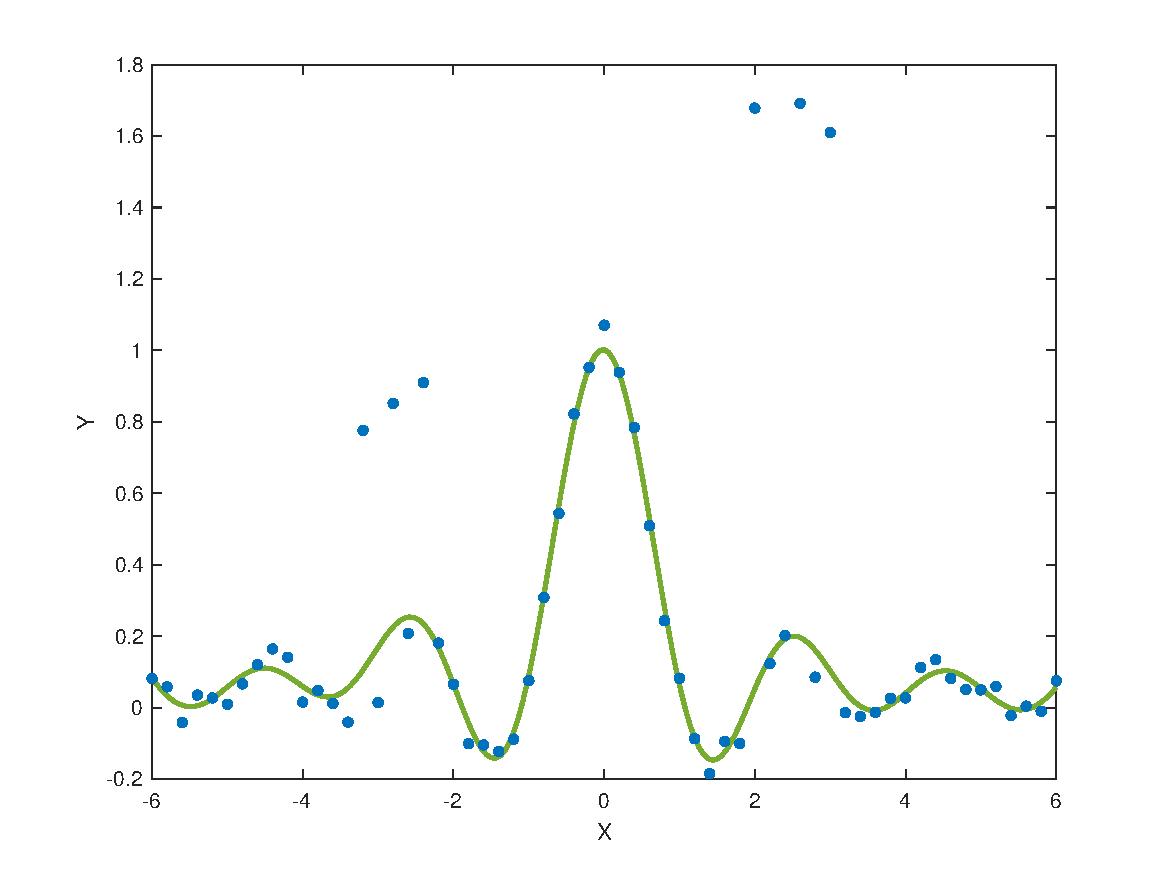
\includegraphics[width=0.3\textwidth]{../src/figures/estimation/robustregression_wlogistic}}\qquad
\subfloat[\textit{Myriad} weight function.]{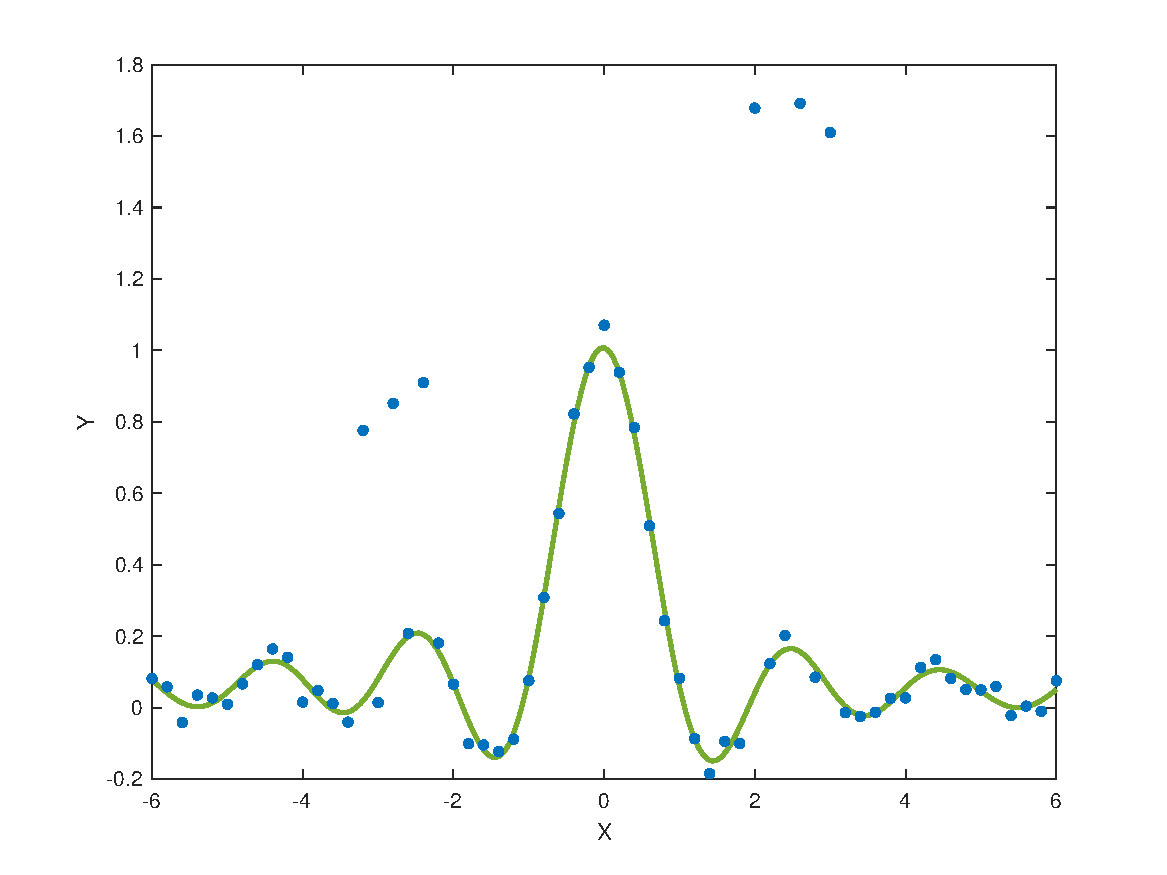
\includegraphics[width=0.3\textwidth]{../src/figures/estimation/robustregression_wmyriad}}
\caption{Comparing non-robust regression to robust regression. A variety of weight functions are considered. The smallest \textit{mse} on the test set was obtained with the \textit{Hampel} weight function. The noise is not normally distributed in contrast with the datasets shown before.}
\label{robustsinc}
\end{figure}

% \fakesubsection{Introduction: time series prediction}{}

\fakesubsection{Logmap dataset}{}

The provided model for predicting measurements for the logmap dataset performs quite badly as can be seen below. The results call for the tuning of the three parameters.

\vspace{0.5cm}
\begin{figure}[!h]
\centering
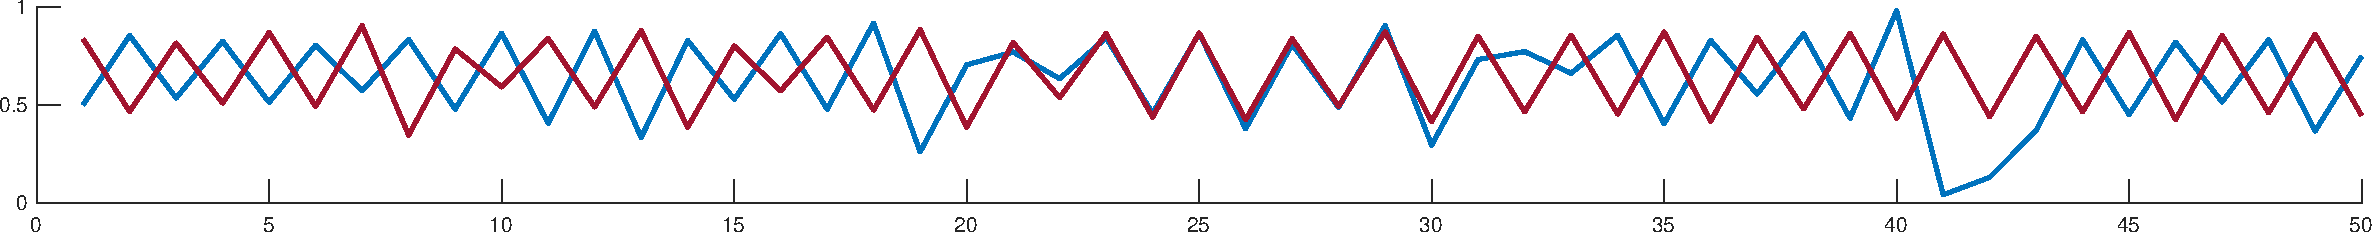
\includegraphics[width=\textwidth]{../src/figures/logmap/init}
\caption{Initial attempt at modelling the logmap dataset (ground truth in blue, prediction in red).}
\label{logmapinit}
\end{figure}

\par A straightforward way of picking a so-called order of a time series model (i.e. the number of past measurements taken into account for prediction of the next measurement) is to take advantage of the fact that the given dataset is rather small and the order is a discrete variable. This makes it sensible to go over all possible orders and tune regularisation parameter $\gamma$ and any of the kernel parameters for every possible order separately.

\begin{figure}[!h]
\centering
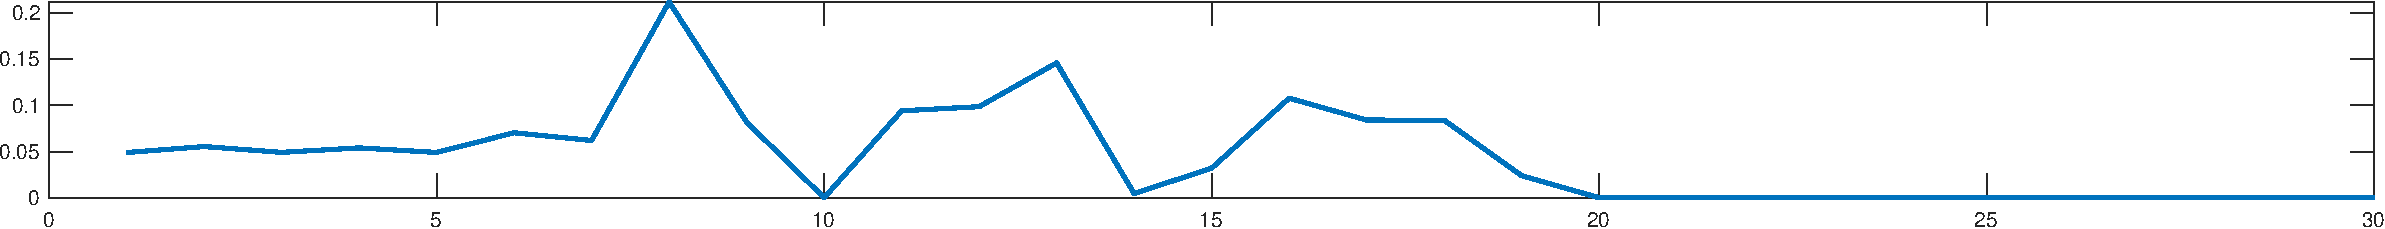
\includegraphics[width=\textwidth]{../src/figures/logmap/mseval}
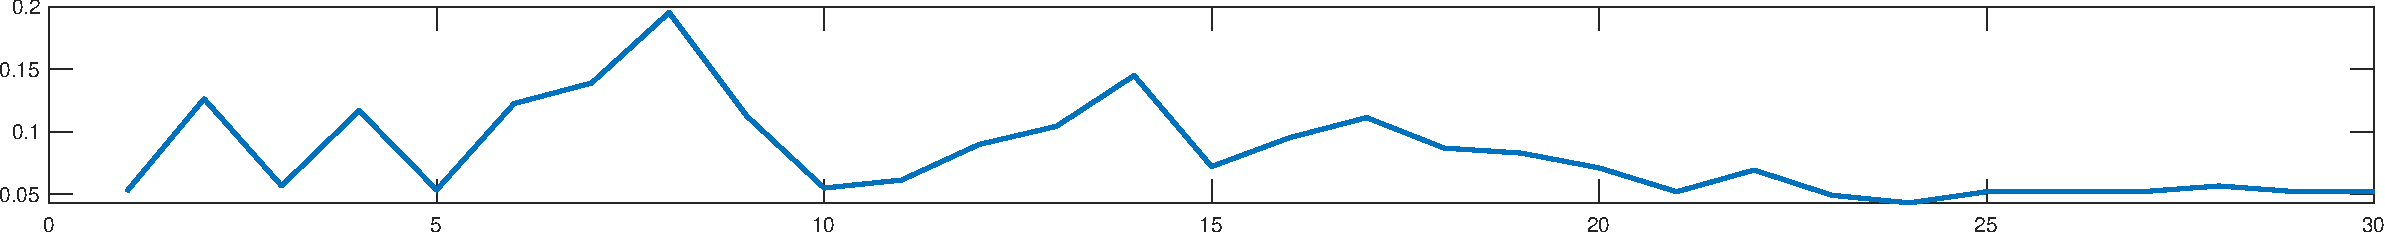
\includegraphics[width=\textwidth]{../src/figures/logmap/msetest}
\caption{Mean squared errors for just one tuned model per possible order. The top row gives the error for the training set, the bottom row for the test set. A minimum is obtained starting at \texttt{order} = 21. The mean absolute errors give a slightly more meaningful picture here because a model predicting the mean value for every time step could have a smaller mean squared error than a more meaningful model (due to the fact that the data lies between 0 and 1).}
\label{logmapord}
\end{figure}

To find good values for the parameters either cross-validation or the Bayesian framework discussed previously can be used. Both methods were tried and the results with the Bayesian framework are shown in figure \ref{logmapord}. In that figure the mean squared errors are plotted in function of the order for LS-SVMs using RBF kernels with tuned parameters. This was measured for the training and the test set. A useful order appeared to lie somewhere in the early 20s and picking anything higher may cause poor generalisation due to overfitting. Results with a model with its order equal to 20 are shown below. The performance has clearly improved.

\begin{figure}[!h]
\centering
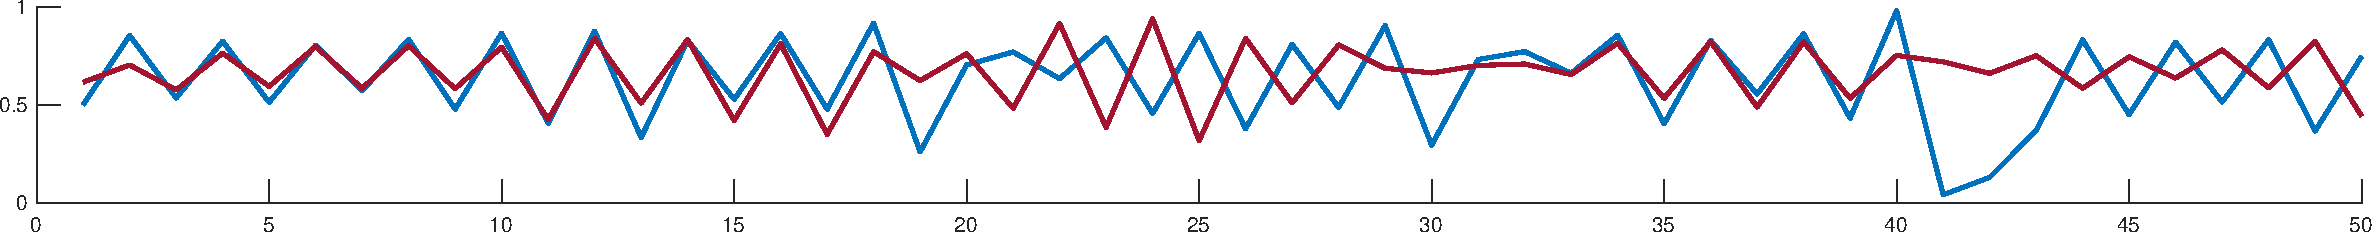
\includegraphics[width=\textwidth]{../src/figures/logmap/final}
\caption{Results for a model using an RBF kernel with tuned parameters. The order is 21, $\gamma\approx 114481.964$ and $\sigma^2\approx 985.571$.}
\label{logmapfinal}
\end{figure}

%It can be noted that the automatic tuning of parameters does not take the simplicity into account, only the error on the validation set. This may lead to rather complex models and poor generalisation performance.

\fakesubsection{Santa Fe dataset}{}

The per-order mean squared errors for an analogous tuning approach applied to the Santa Fe dataset (this time by using cross-validation rather than making use of the Bayesian network) are shown in figure \ref{santafeord}.

\begin{figure}[!h]
\centering
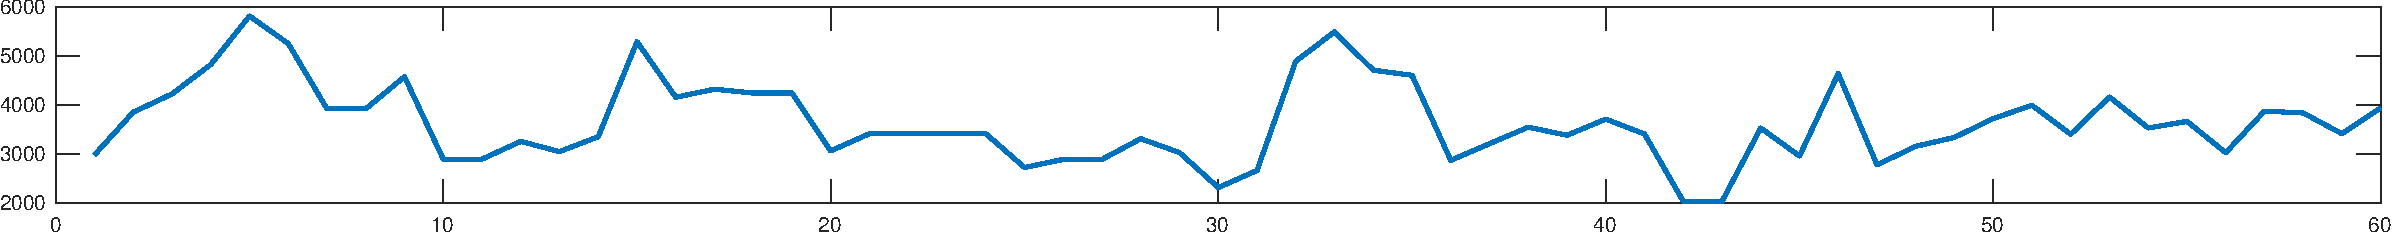
\includegraphics[width=\textwidth]{../src/figures/santafe/mseval}
%\includegraphics[width=\textwidth]{../src/figures/santafe/msestest}
\caption{Mean squared errors for various models in function of the order. Parameters were tuned automatically using a grid search. Outliers (large errors) are `ignored' (i.e. set equal to the error for the previous order) to improve the visualisation.}
\label{santafeord}
\end{figure}

Picking the model with lowest error (prioritising a small order) gave the following result :

\begin{figure}[!h]
\centering
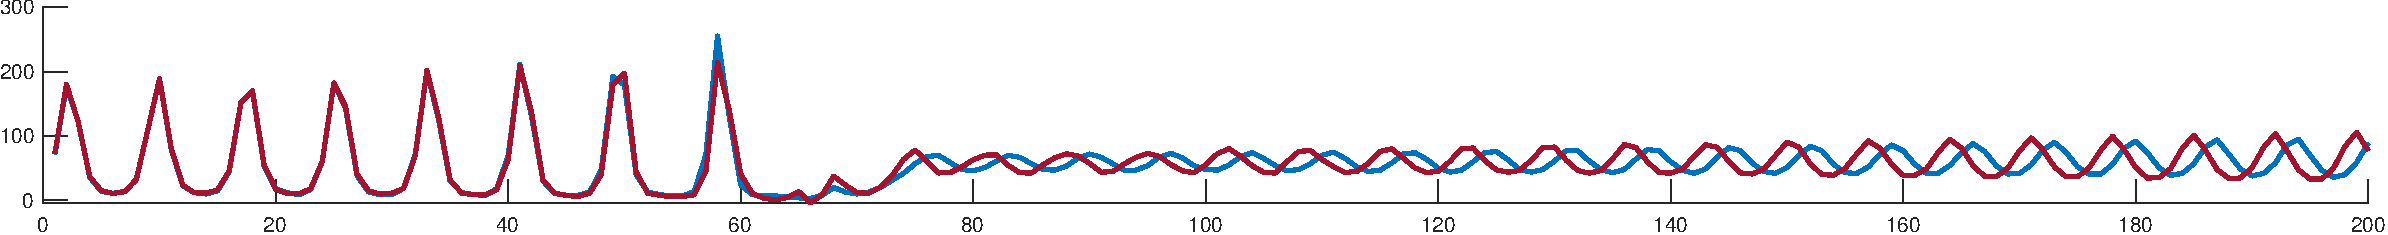
\includegraphics[width=\textwidth]{../src/figures/santafe/final}
\caption{Results for a model using an RBF kernel with tuned parameters. The order is 42, $\gamma\approx 8423.289$ and $\sigma^2\approx 14.017$.}
\label{santafefinal}
\end{figure}

Due to the limited number of runs the whole tuning procedure by no means proves that this model is best or that this order is optimal. By doing more experiments confidence can grow that certain orders are optimal for this particular dataset. 

\par Up til now only LS-SVMs were toyed with. It's also possible to work with classical SVMs which - due to the choice of loss function - provide sparsity without necessitating a pruning post-processing step or some other approach to enforce it. Using \texttt{scikit-learn} a script was built to do classical SVM regression using the \texttt{SVR} class. Grid search was done to tune the parameters of an RBF kernel first, which proved to be equivalent to the LS-SVM result while having less support vectors. An attempt was made at using an other kernel called the ANOVA kernel which is said to perform well in the case of multivariate regression problems, but despite some limited tuning (with a grid search) the results weren't close to those of the RBF kernel. The sparsity of the classical SVMs with RBF kernels wasn't impressive ; about 90\% of the training set was kept. Other strategies such as LSTMs are always possible as well though the obtained results appear quite satisfactory.